\section{Objective 1: \texttt{mpbenchmark}}

Results from the proposed solution collected from desktop(\texttt{x86} processor) are shown below, they are presented in the legend ``C++" and ``C++(SIMD Optimised)". A benchmark plot along with a speedup plot are shown in figures ~\ref{fig:mpbenchmark_desktop_plot} and ~\ref{fig:mpbenchmark_desktop_speedup_plot} respectively. Full system specifications of the desktop(\texttt{x86}) along with the Raspberry Pi processors can be found in the appendix.

\begin{figure}[htbp] % Positioning preference: here, top, bottom, page
	\centering
	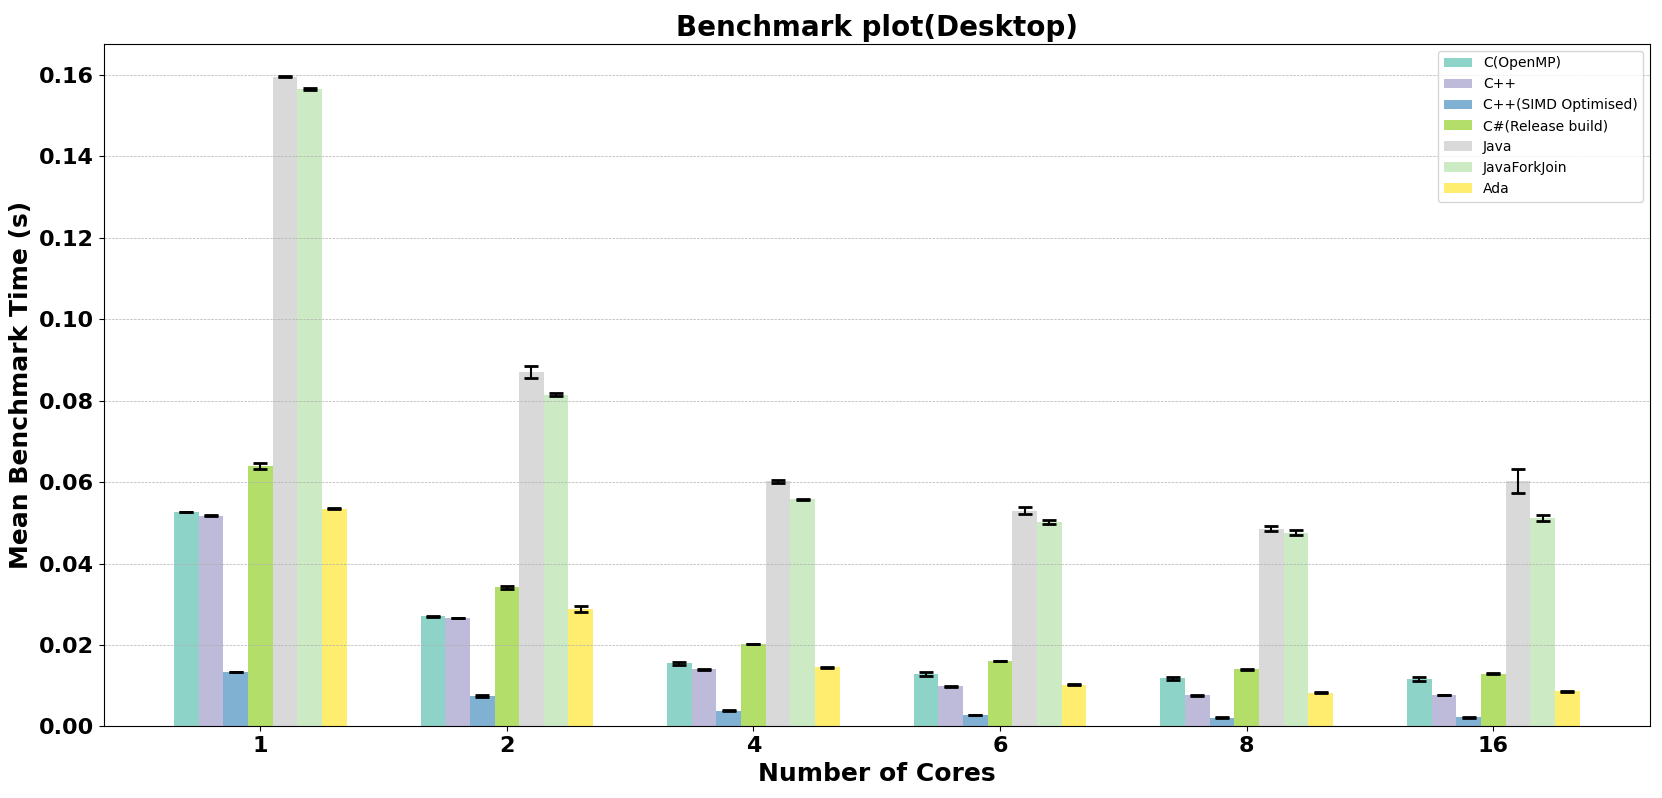
\includegraphics[width=1\textwidth, height=20cm]{~/Documents/Part_D_Modules/Individual_Project/Individual_report/figures/mpbenchmark_desktop.png} % Adjust the path and width as needed
	\caption{Mean benchmark plot of \texttt{mpbenchmark} collected from \texttt{x86} processor in seconds. The error bars represent 95\% confidence interval. (Lower is better).}
	\label{fig:mpbenchmark_desktop_plot} % Use this label to reference the figure
\end{figure}


\begin{figure}[htbp] % Positioning preference: here, top, bottom, page
	\centering
	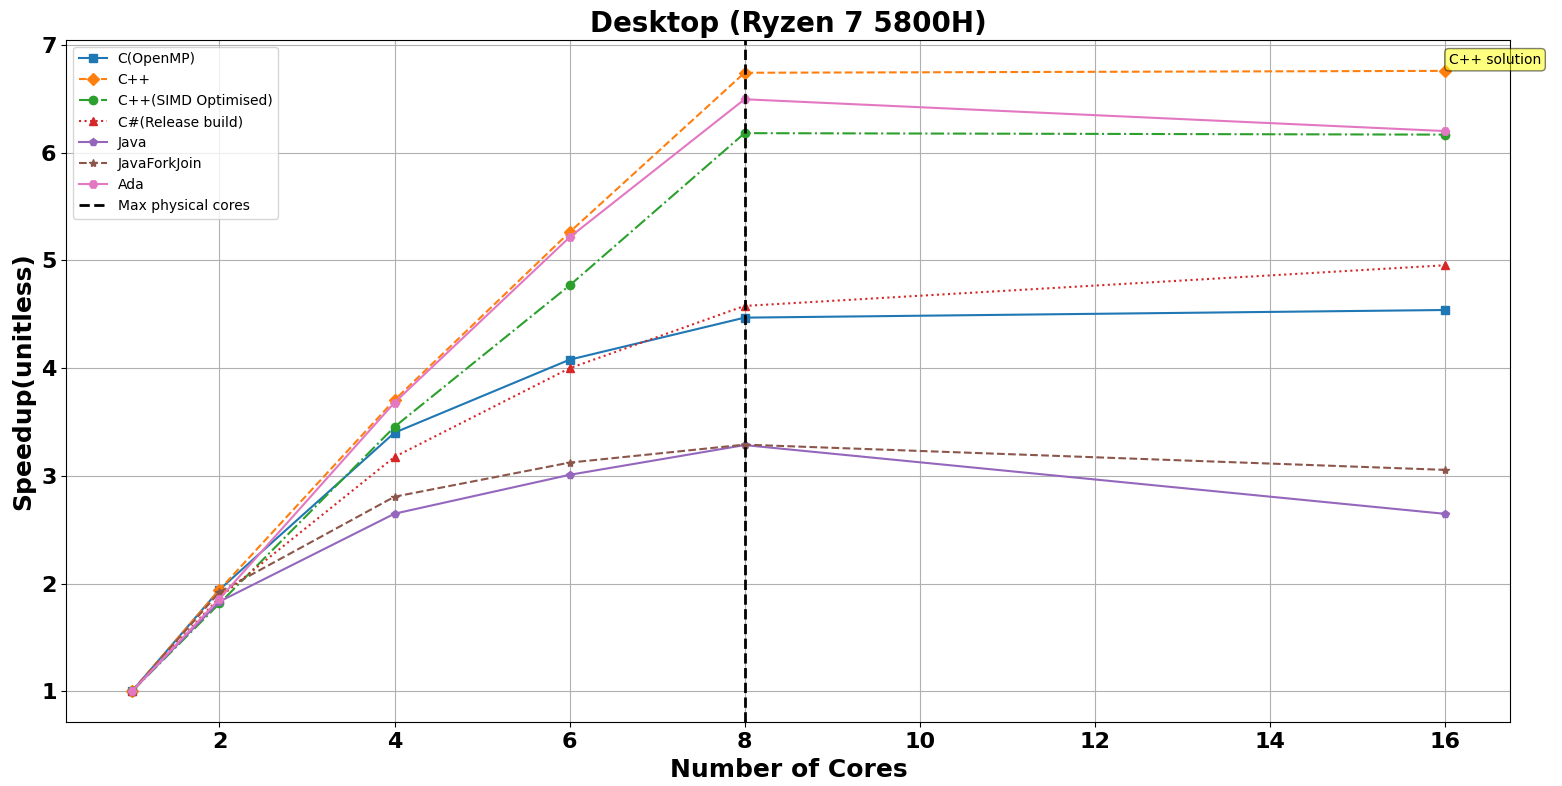
\includegraphics[width=1\textwidth, height=20cm]{~/Documents/Part_D_Modules/Individual_Project/Individual_report/figures/mpbenchmark_desktop_speedup.png} % Adjust the path and width as needed
	\caption{Speedup plot collected from \texttt{x86} processor. The vertical black line shows the maximum physical cores of the processor. (Higher is better).}
	\label{fig:mpbenchmark_desktop_speedup_plot} % Use this label to reference the figure
\end{figure}

On desktop(\texttt{x86}) processor, \texttt{AVX2} instructions were used to implement SIMD intrinsics therefore we compare the decimal precision with the original unoptimised SIMD code, see table ~\ref{tab:c++_avx2_pi}.

\begin{table}[htbp]
	\centering
	\begin{tabular}{|c|c|c|}
		\hline
		\textbf{Programming language/configuration} & \textbf{Decimal value of $\pi$} & \textbf{Mean run time using maximum threads(s)} \\ \hline
		\texttt{C++}             & 3.1415926535897643 &  0.007659 \\ \hline
		\texttt{C++/AVX2}   & 3.1415926535899033 &  0.002173  \\ \hline
		\texttt{C}                 & 3.1415926535897643 & 0.011577 \\ \hline
		\texttt{Ada}             & 3.1415926535897643 &  0.008623\\ \hline
	\end{tabular}
	\label{tab:c++_avx2_pi}
	\caption{Comparing the decimal precision of the \texttt{AVX2} enhanced solution with the original.}
\end{table}

% Talk about C++ solution outperforming the original in both run times and speedup 
% C++ SIMD enhanced outperformed even more with a lower speedup.
% Talk about SMT's benefits if any
% Discuss AVX2's decimal precision

The proposed \texttt{C++} solution outperformed the original implementations in \texttt{C} and \texttt{Ada} by over 11\%, marking a significant reduction in runtime. Additionally, it achieved a higher speed-up compared to the \texttt{Ada} solution, as illustrated in figure~\ref{fig:mpbenchmark_desktop_speedup_plot}. The SIMD-enhanced solution achieved a remarkable runtime reduction of over 70\%, significantly outperforming all other solutions. However, this version did not show as large a speedup when run with an increased number of threads, which is not surprising given the already low runtime with a single thread. Moreover, the \texttt{AVX2}-enhanced code demonstrated decimal precision up to 12 decimal places, with discrepancies appearing from the 13th decimal place onwards, as shown in table~\ref{tab:c++_avx2_pi}. This suggests a slight consideration that using \texttt{AVX2} instructions might lead to reduced precision for calculations requiring high decimal accuracy. However, the reduction in decimal precision has been minor, and its effects on the application have been largely inconsequential. Given the dramatic improvement in performance with \texttt{AVX2} instructions, the minor loss of decimal precision seems negligible compared to the benefits. Both solutions have met their objectives, with the first achieving superior speed-up and the second providing insights into CPU performance when SIMD intrinsics are utilized.

Another noteworthy observation is the lack of performance gain when scaling from 8 to 16 cores. The processor used supports simultaneous multi-threading (SMT), commonly branded as ``Hyper-threading" for Intel CPUs, which is typical in modern \texttt{x86} processors. SMT theoretically allows each physical core to execute two threads, and an 8-core processor with SMT would appear to have 16 cores. However, the proposed solutions, along with other compiled languages like \texttt{C} and \texttt{Ada}, showed negligible performance gains by utilizing the virtual cores. \texttt{Java} experienced a slight performance degradation, while \texttt{C\#} was the only language to demonstrate a performance increase. Using the results from the \texttt{x86} processor, we can conclude that the additional cores provided by SMT did not enhance performance and, in some cases, even degraded it.

Results obtained from the latest Raspberry Pi 5 (\texttt{Cortex A-76} processor) are shown in figures ~\ref{fig:mpbenchmark_rpi5_plot} and ~\ref{fig:mpbenchmark_rpi5_speedup_plot}. The results obtained from the Raspberry Pi 4(\texttt{Cortex A-72} processor) are shown in figures ~\ref{fig:mpbenchmark_rpi4_plot} and ~\ref{fig:mpbenchmark_rpi4_speedup_plot}.

\begin{figure}[htbp] % Positioning preference: here, top, bottom, page
	\centering
	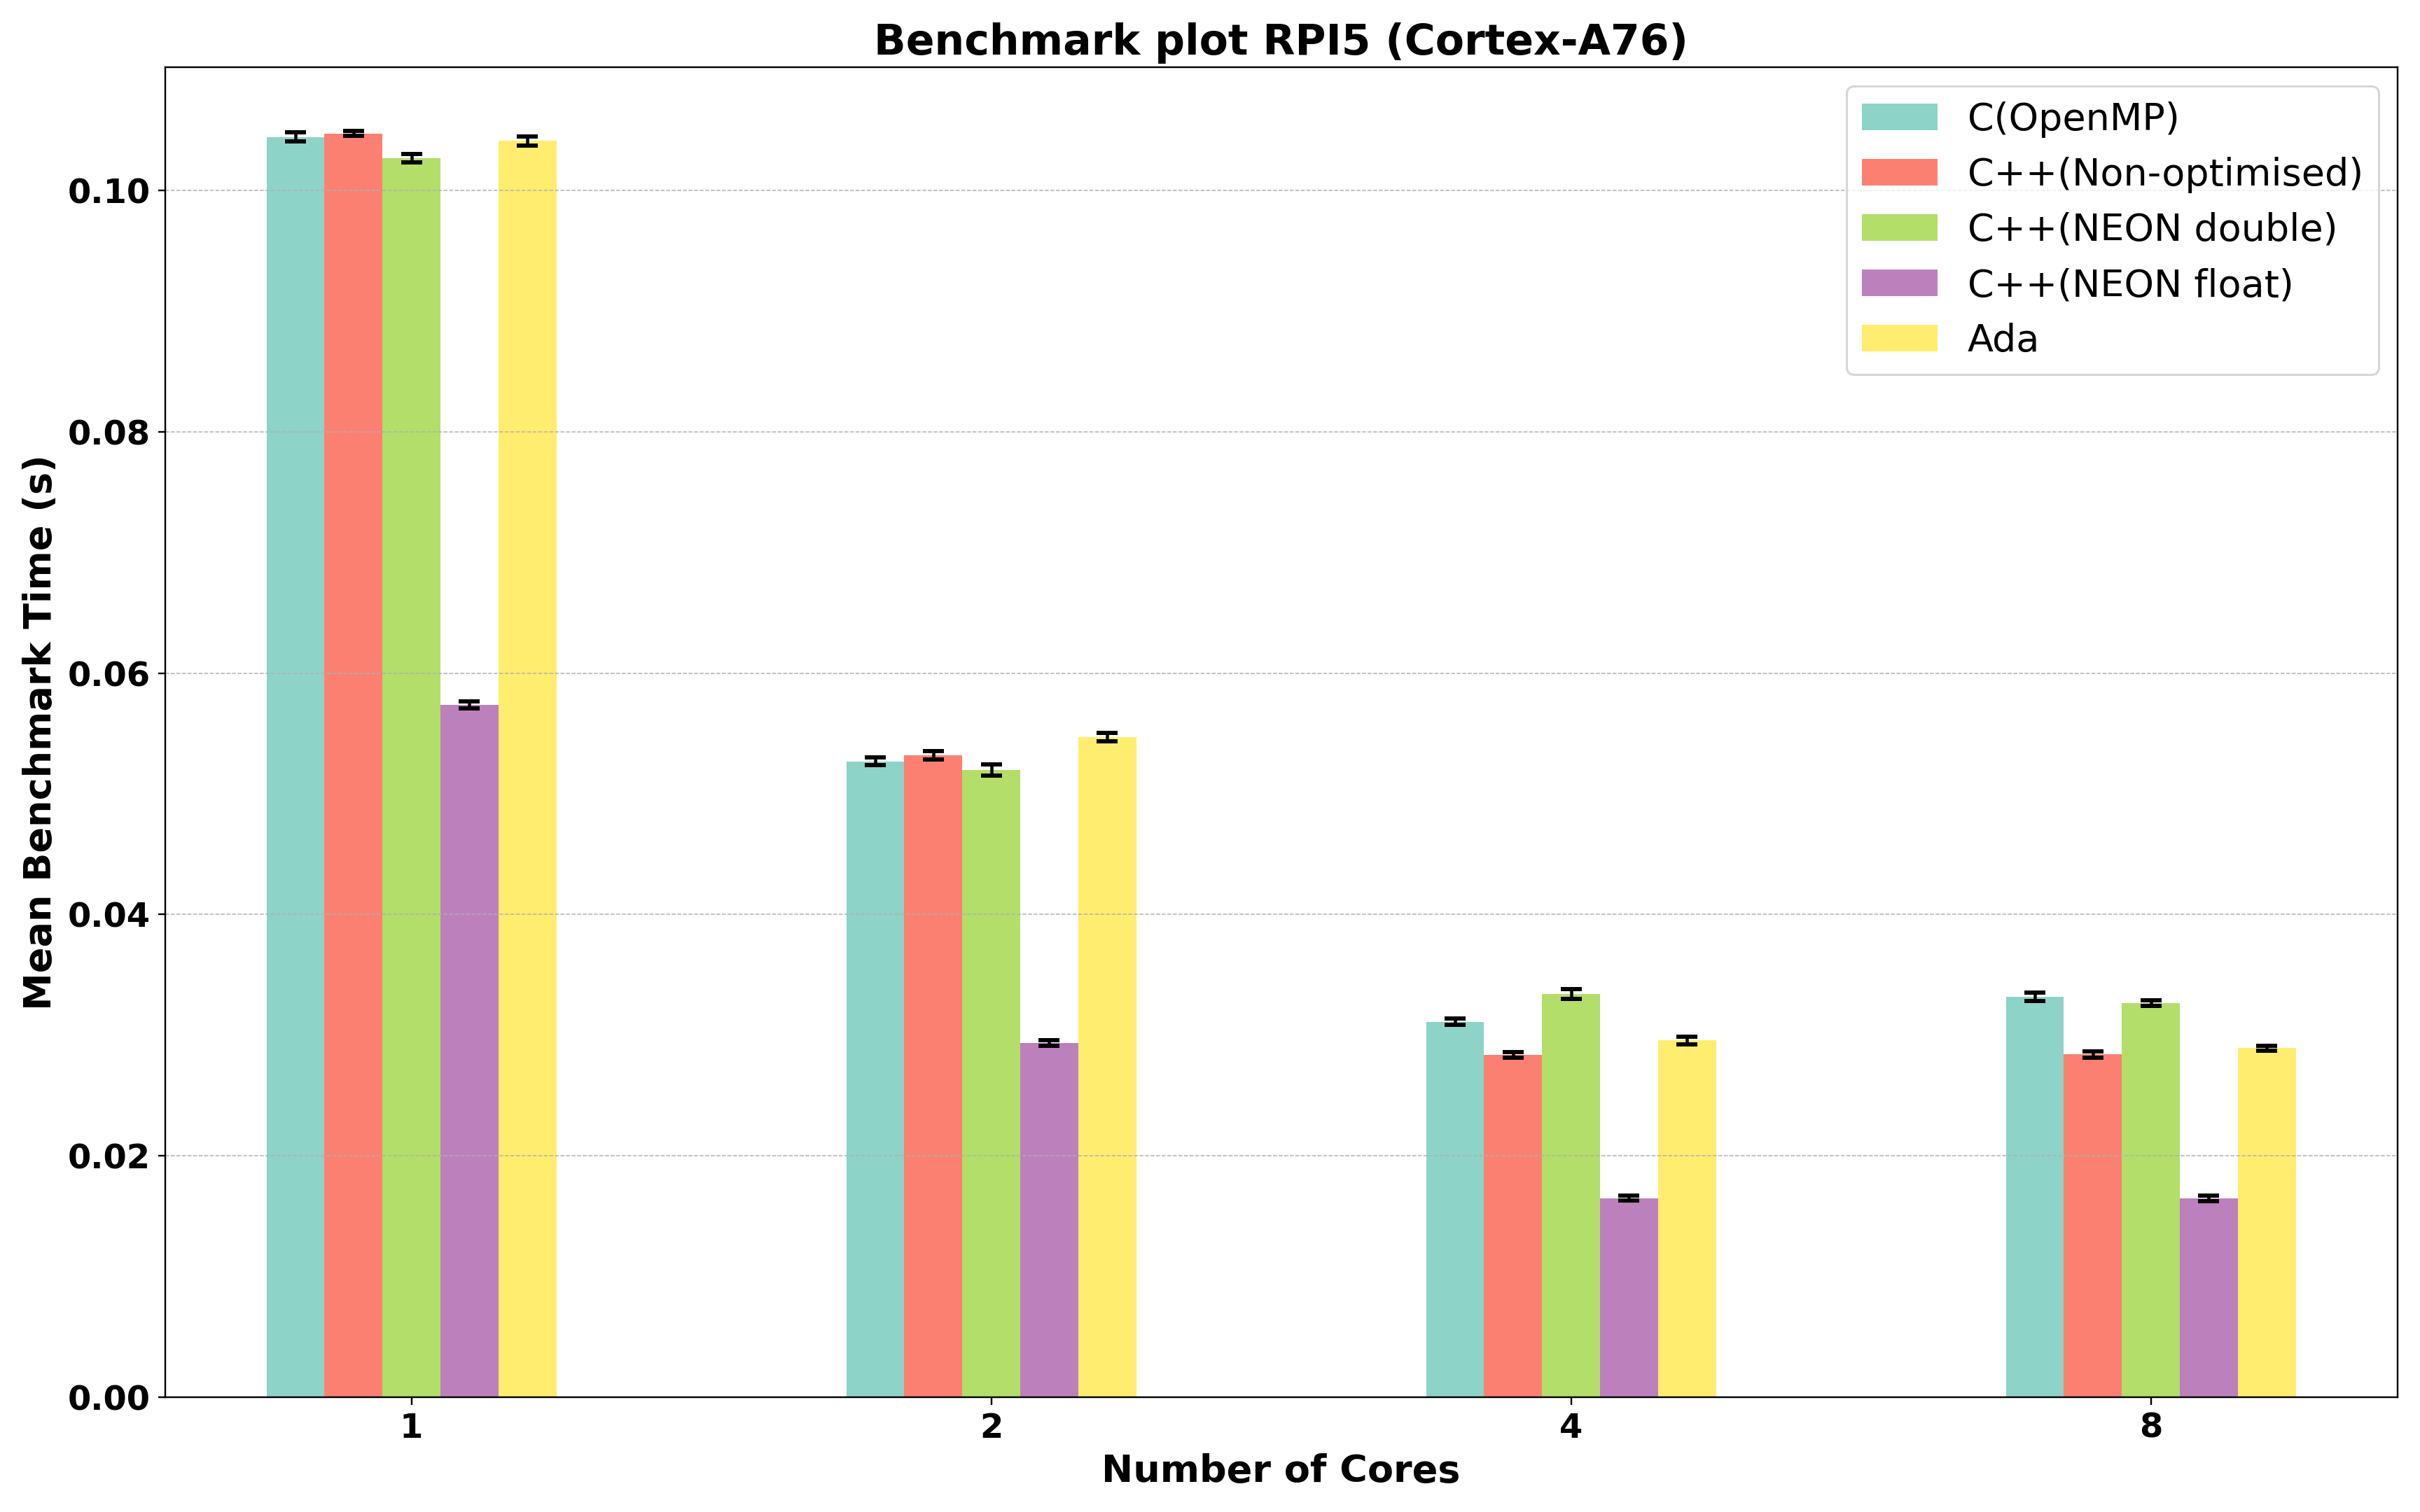
\includegraphics[width=1\textwidth, height=20cm]{~/Documents/Part_D_Modules/Individual_Project/Individual_report/figures/mpbenchmark_rpi5.png} % Adjust the path and width as needed
	\caption{Mean benchmark plot of results collected from Raspberry Pi 5(in seconds). The error bars represent 95\% confidence interval. (Lower is better).}
	\label{fig:mpbenchmark_rpi5_plot} % Use this label to reference the figure
\end{figure}

\begin{figure}[htbp] % Positioning preference: here, top, bottom, page
	\centering
	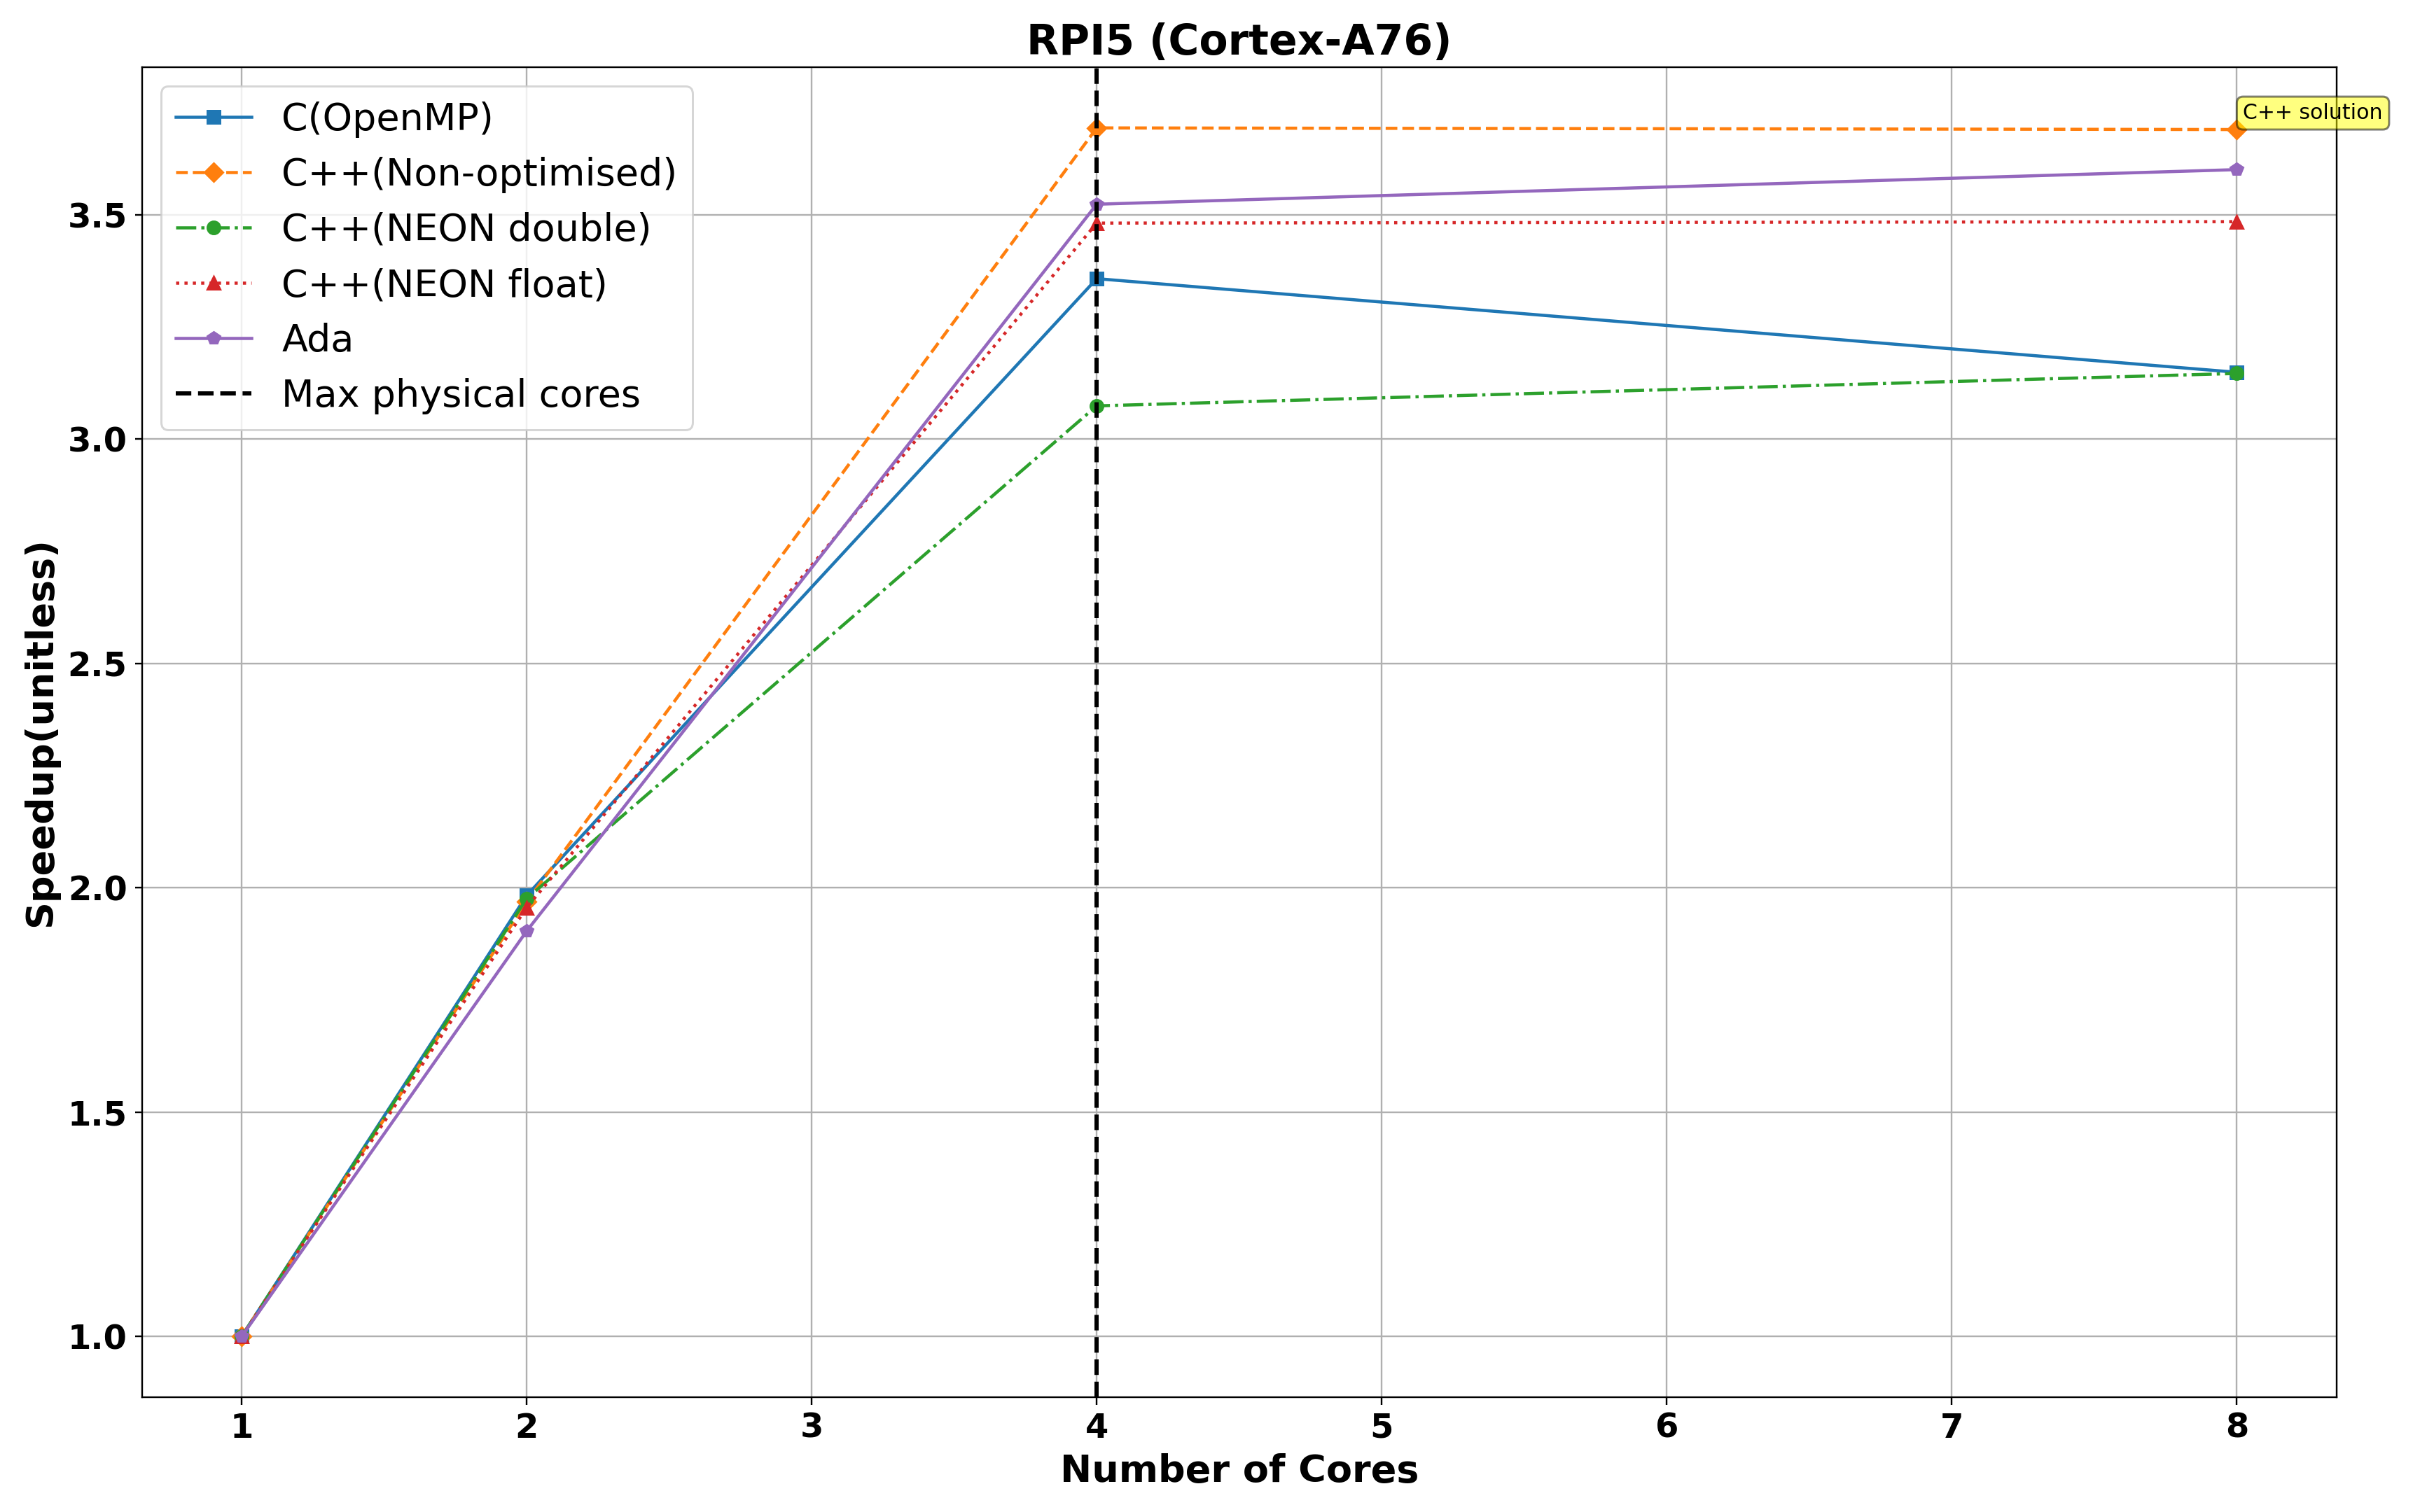
\includegraphics[width=1\textwidth, height=20cm]{~/Documents/Part_D_Modules/Individual_Project/Individual_report/figures/mpbenchmark_rpi5_speedup.png} % Adjust the path and width as needed
	\caption{Speedup plot collected from Raspberry Pi 5 processor. The vertical black line shows the maximum physical cores of the processor. (Higher is better).}
	\label{fig:mpbenchmark_rpi5_speedup_plot} % Use this label to reference the figure
\end{figure}

\begin{figure}[htbp] % Positioning preference: here, top, bottom, page
	\centering
	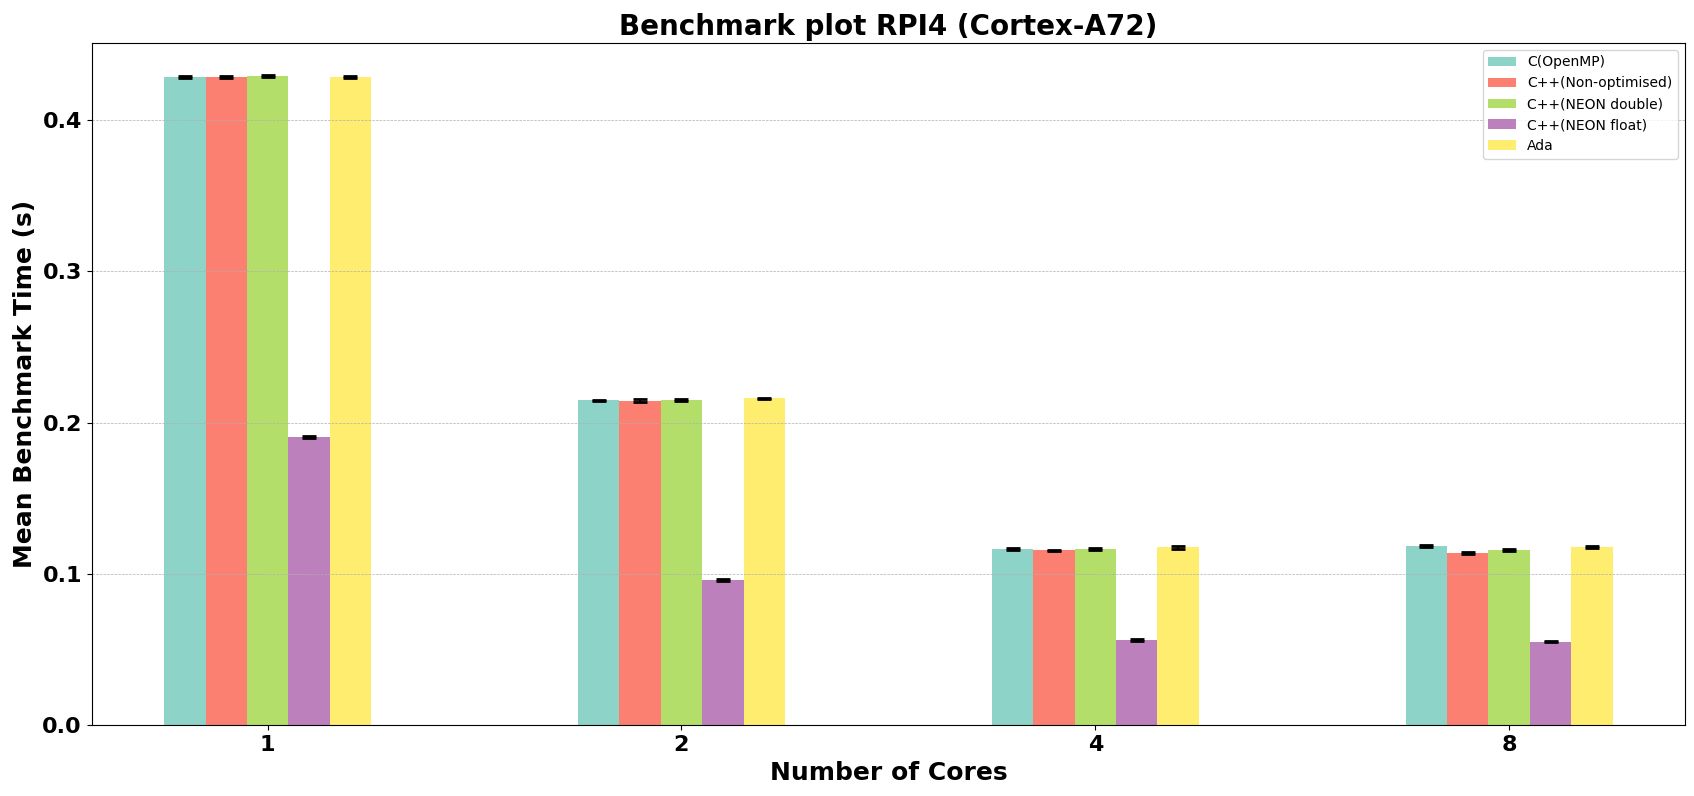
\includegraphics[width=1\textwidth, height=20cm]{~/Documents/Part_D_Modules/Individual_Project/Individual_report/figures/mpbenchmark_rpi4.png} % Adjust the path and width as needed
	\caption{Mean benchmark plot of results collected from Raspberry Pi 4(in seconds). The error bars represent 95\% confidence interval. (Lower is better).}
	\label{fig:mpbenchmark_rpi4_plot} % Use this label to reference the figure
\end{figure}

\begin{figure}[htbp] % Positioning preference: here, top, bottom, page
	\centering
	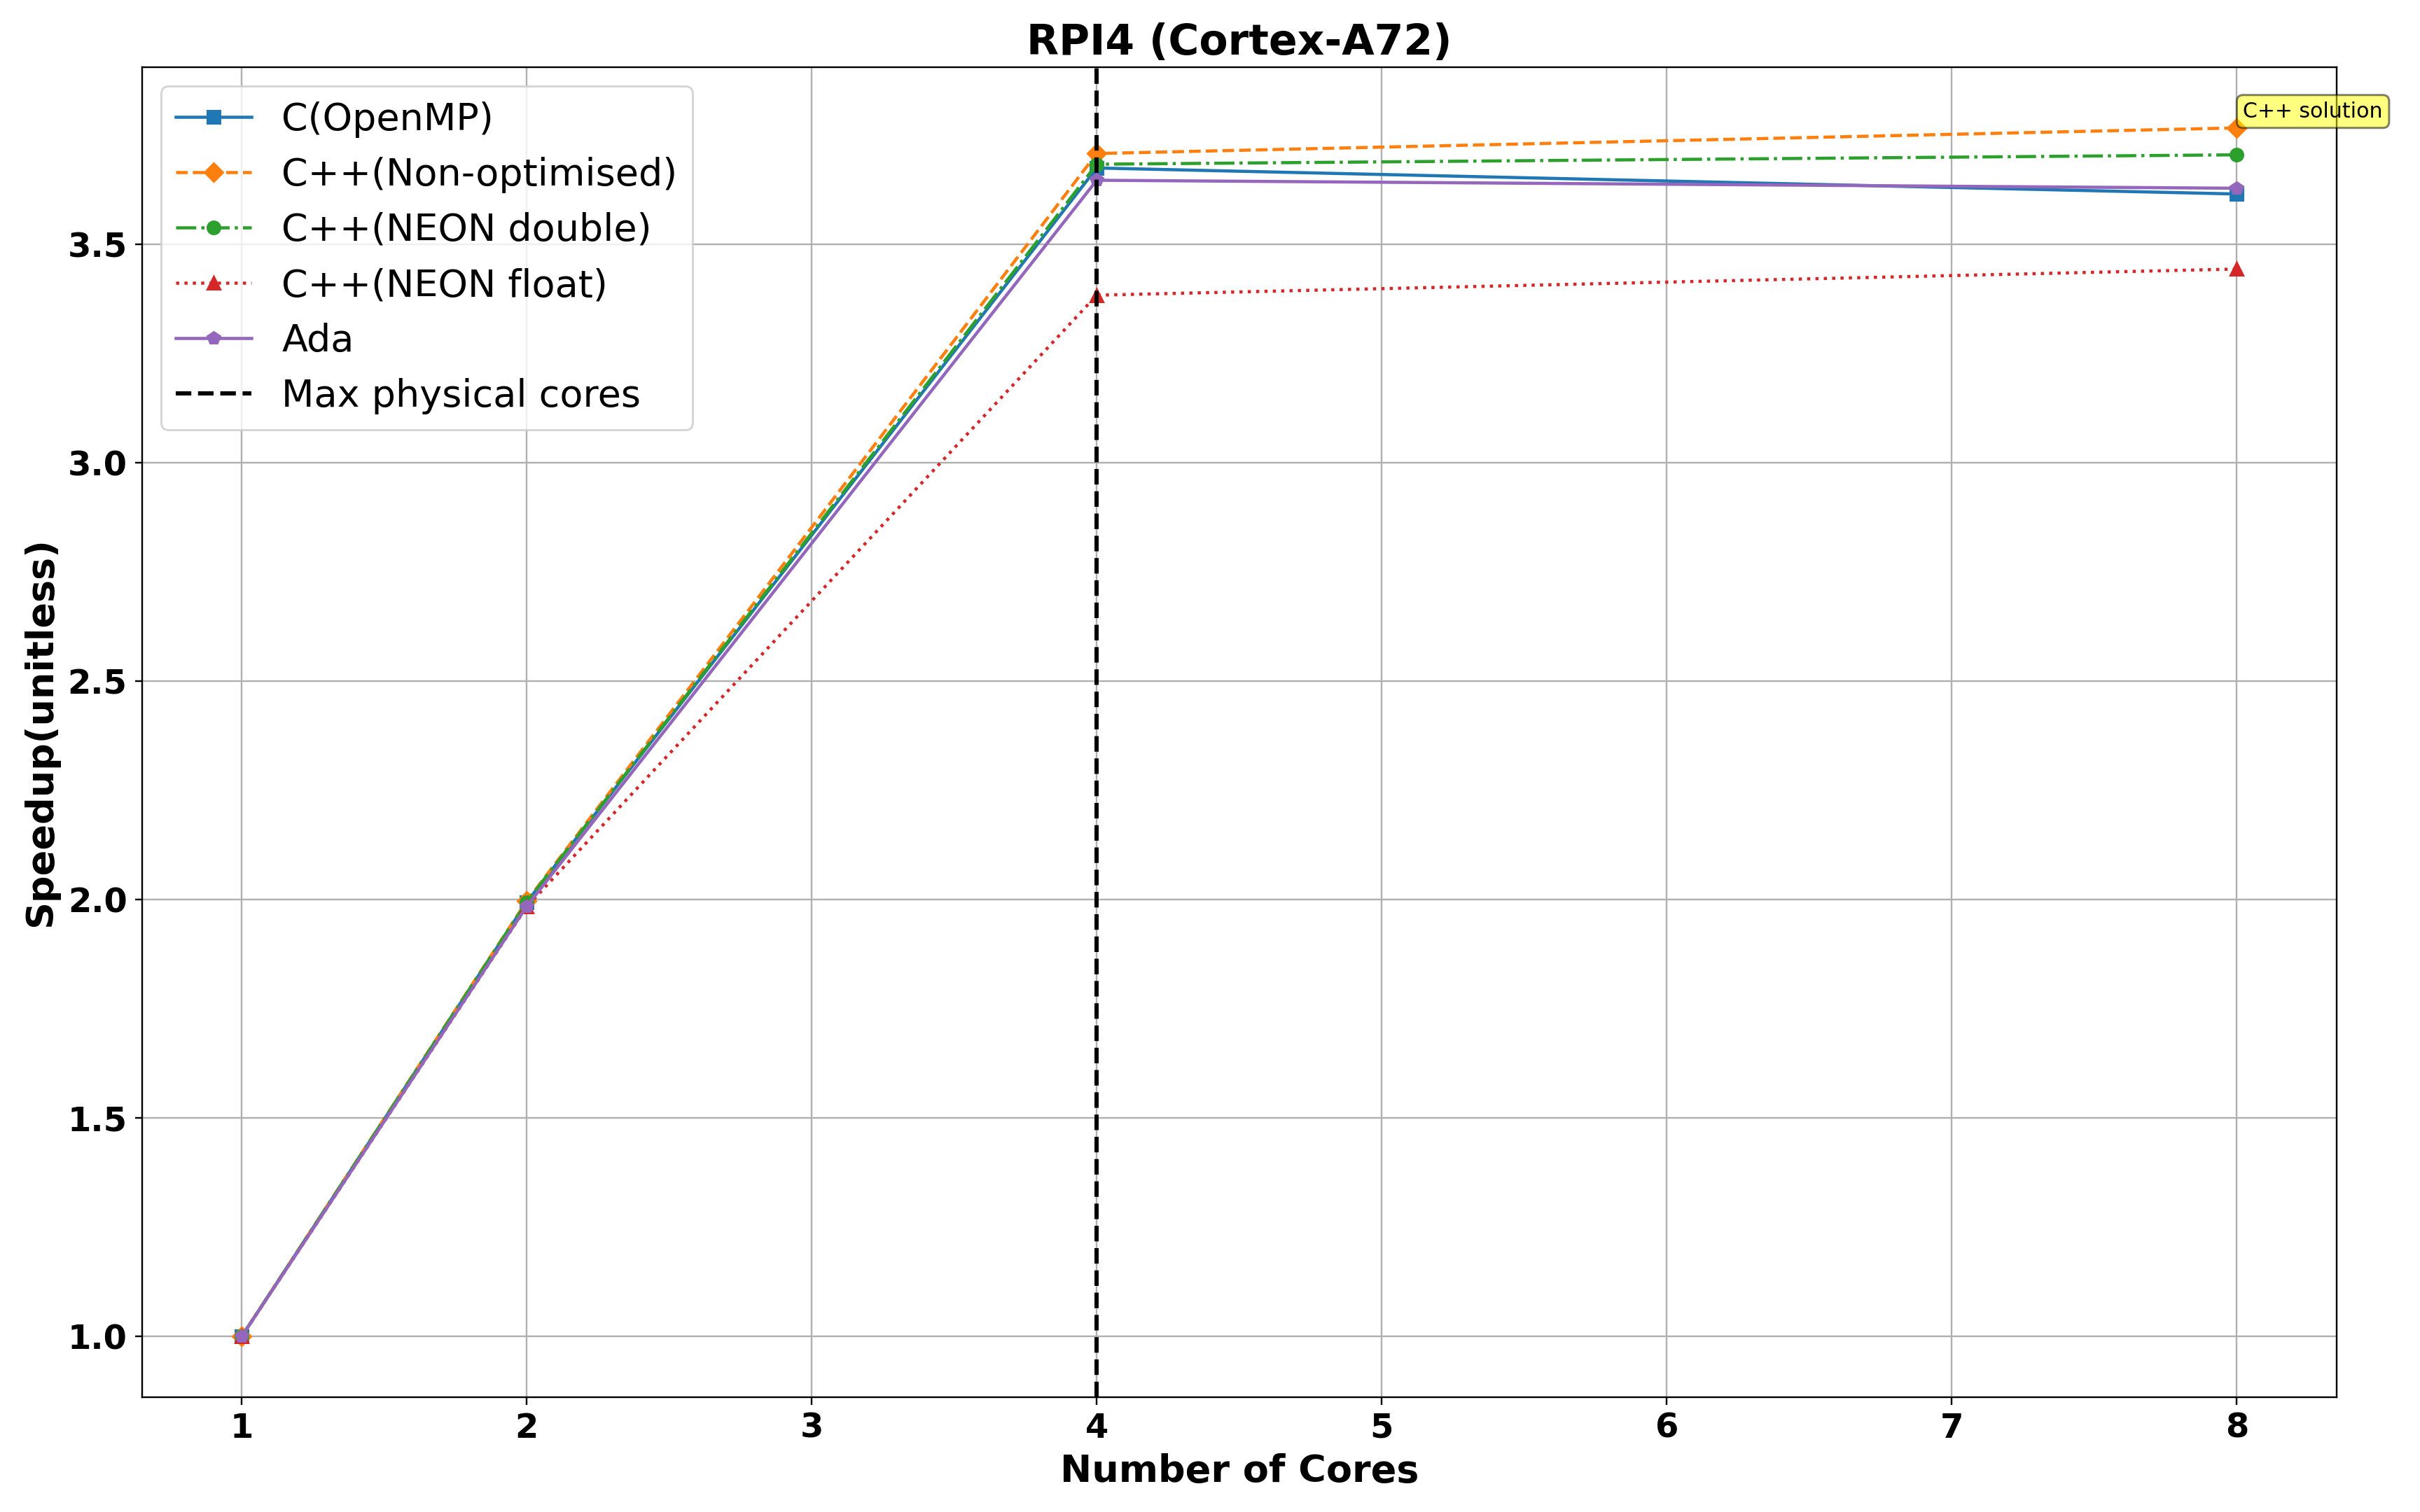
\includegraphics[width=1\textwidth, height=20cm]{~/Documents/Part_D_Modules/Individual_Project/Individual_report/figures/mpbenchmark_rpi4_speedup.png} % Adjust the path and width as needed
	\caption{Speedup plot collected from Raspberry Pi 4 processor. The vertical black line shows the maximum physical cores of the processor. (Higher is better).}
	\label{fig:mpbenchmark_rpi4_speedup_plot} % Use this label to reference the figure
\end{figure}

The decimal precision of using single and double precision floating point \texttt{NEON} instructions on the Raspberry Pi processors is compared in table ~\ref{tab:c++_neon_pi}.

\begin{table}[htbp]
	\centering
	\begin{tabular}{|c|c|c|c|}
		\hline
		\textbf{Programming language/configuration} & \textbf{Decimal value of $\pi$} & \textbf{Run time RPI5(s)} & \textbf{Run time RPI4(s)} \\ \hline
		\texttt{C++}                                                   & 3.1415926535897643 & 0.028356  & 0.115569 \\ \hline
		\texttt{C++/single-precision NEON}              & 3.141531467437744   &  0.016477 & 0.056352 \\ \hline
		\texttt{C++/double-precision NEON}             & 3.14159265358986     & 0.033399  & 0.116423 \\ \hline
		\texttt{C}                                                        & 3.1415926535897643 & 0.031107  & 0.116538\\ \hline 
		\texttt{Ada}                                                    & 3.1415926535897643  & 0.029549  & 0.117536 \\ \hline
	\end{tabular}
	\label{tab:c++_neon_pi}
	\caption{Comparing the decimal precision of the \texttt{NEON} enhanced solutions. RPI5 - Raspberry Pi 5, RPI4- Raspberry Pi 4. Mean benchmark time in seconds collected using maximum cores on the system(4 cores).}
\end{table}

% Talk about the proposed solution's performance in PI5 and PI4. 
% Talk about the speedup
% Talk about NEON solutions and their respective decimal precision.
% Can include the comparision with other solutions in the appendix, like Java and C# and Raspberry Pi 3 

The proposed solution outperformed both the \texttt{C} and \texttt{Ada} solutions in terms of runtime and speedup. On the Raspberry Pi 5, a slight reduction in runtime (about 4\%) and a notable improvement in speedup were observed. The results on the Raspberry Pi 4 were less impressive, showing only a 1\% improvement in performance and a marginal increase in speedup. Nevertheless, the proposed \texttt{C++} solution outperformed the original solutions in terms of runtime and speedup on both Raspberry Pi devices, although the improvement was marginal on the Raspberry Pi 4.

The \texttt{NEON} enhanced solutions using single precision floating-point produced over a 40\% reduction in time at the cost of lower speedup across threads and a reduced decimal precision to four decimal places. On the Raspberry Pi 5, the \texttt{NEON} solution using double precision failed to reduce runtime and produced the worst overall speedup across varying numbers of threads. On the Raspberry Pi 4, the \texttt{NEON} double precision solution did not reduce the runtime and produced a similar speedup to other solutions. However, the double precision solutions did offer far superior decimal precision, up to 12 decimal places. Given \texttt{NEON} instructions' reduced support for double precision floating points, developers must choose between single precision for significantly improved performance but lower decimal precision, and double precision, which did not improve performance on the tested embedded processors. These results are summarized in table~\ref{tab:c++_neon_pi}.

Benchmarks allow us to compare the latest Raspberry Pi 5 (\texttt{Cortex A-76}) against the older Raspberry Pi 4 (\texttt{Cortex A-72}). The \texttt{Cortex A-76} performed 75\% faster in terms of runtime when comparing the proposed \texttt{C++} solution, roughly \texttt{4x} faster. The \texttt{Cortex A-76} processor offered a 42\% reduction in runtime when \texttt{NEON(float)} enhanced code was used compared to a 51\% reduction in runtime for the \texttt{Cortex A-72}. Both processors exhibited a lower speedup when \texttt{NEON} instructions were used, similar to what was observed with the \texttt{x86} processor. The superior performance of the \texttt{Cortex A-76} may be attributed to a faster clock speed of 2.4 GHz compared to the 1.5GHz of the older \texttt{Cortex A-72} \cite{rasp_pi5_pi4_comparision}.

The proposed \texttt{C++} solution surpassed the previously developed \texttt{mpbenchmark}\cite{mpbenchmark_paper} on both \texttt{x86} and \texttt{ARM} processors. It offered better speedup across threads, and an alternate novel \texttt{SIMD} enhanced version (where the application decides whether to use \texttt{AVX2} or \texttt{NEON} depending on the processor type) can be utilized to analyse the CPUs' SIMD performance and scalability. This unprecedented improvement is part of an upcoming publication.

\section{Objective 2: \texttt{MobileNet}}
After parallelising \texttt{MobileNet} the results collected from desktop(\texttt{x86} processor) were compared with SIMD optimisations and without them. The benchmark and speedup plot are shown in figures ~\ref{fig:mobilenet_desktop_plot} and ~\ref{fig:mobilenet_desktop_speedup}. 

\begin{figure}[htbp] % Positioning preference: here, top, bottom, page
	\centering
	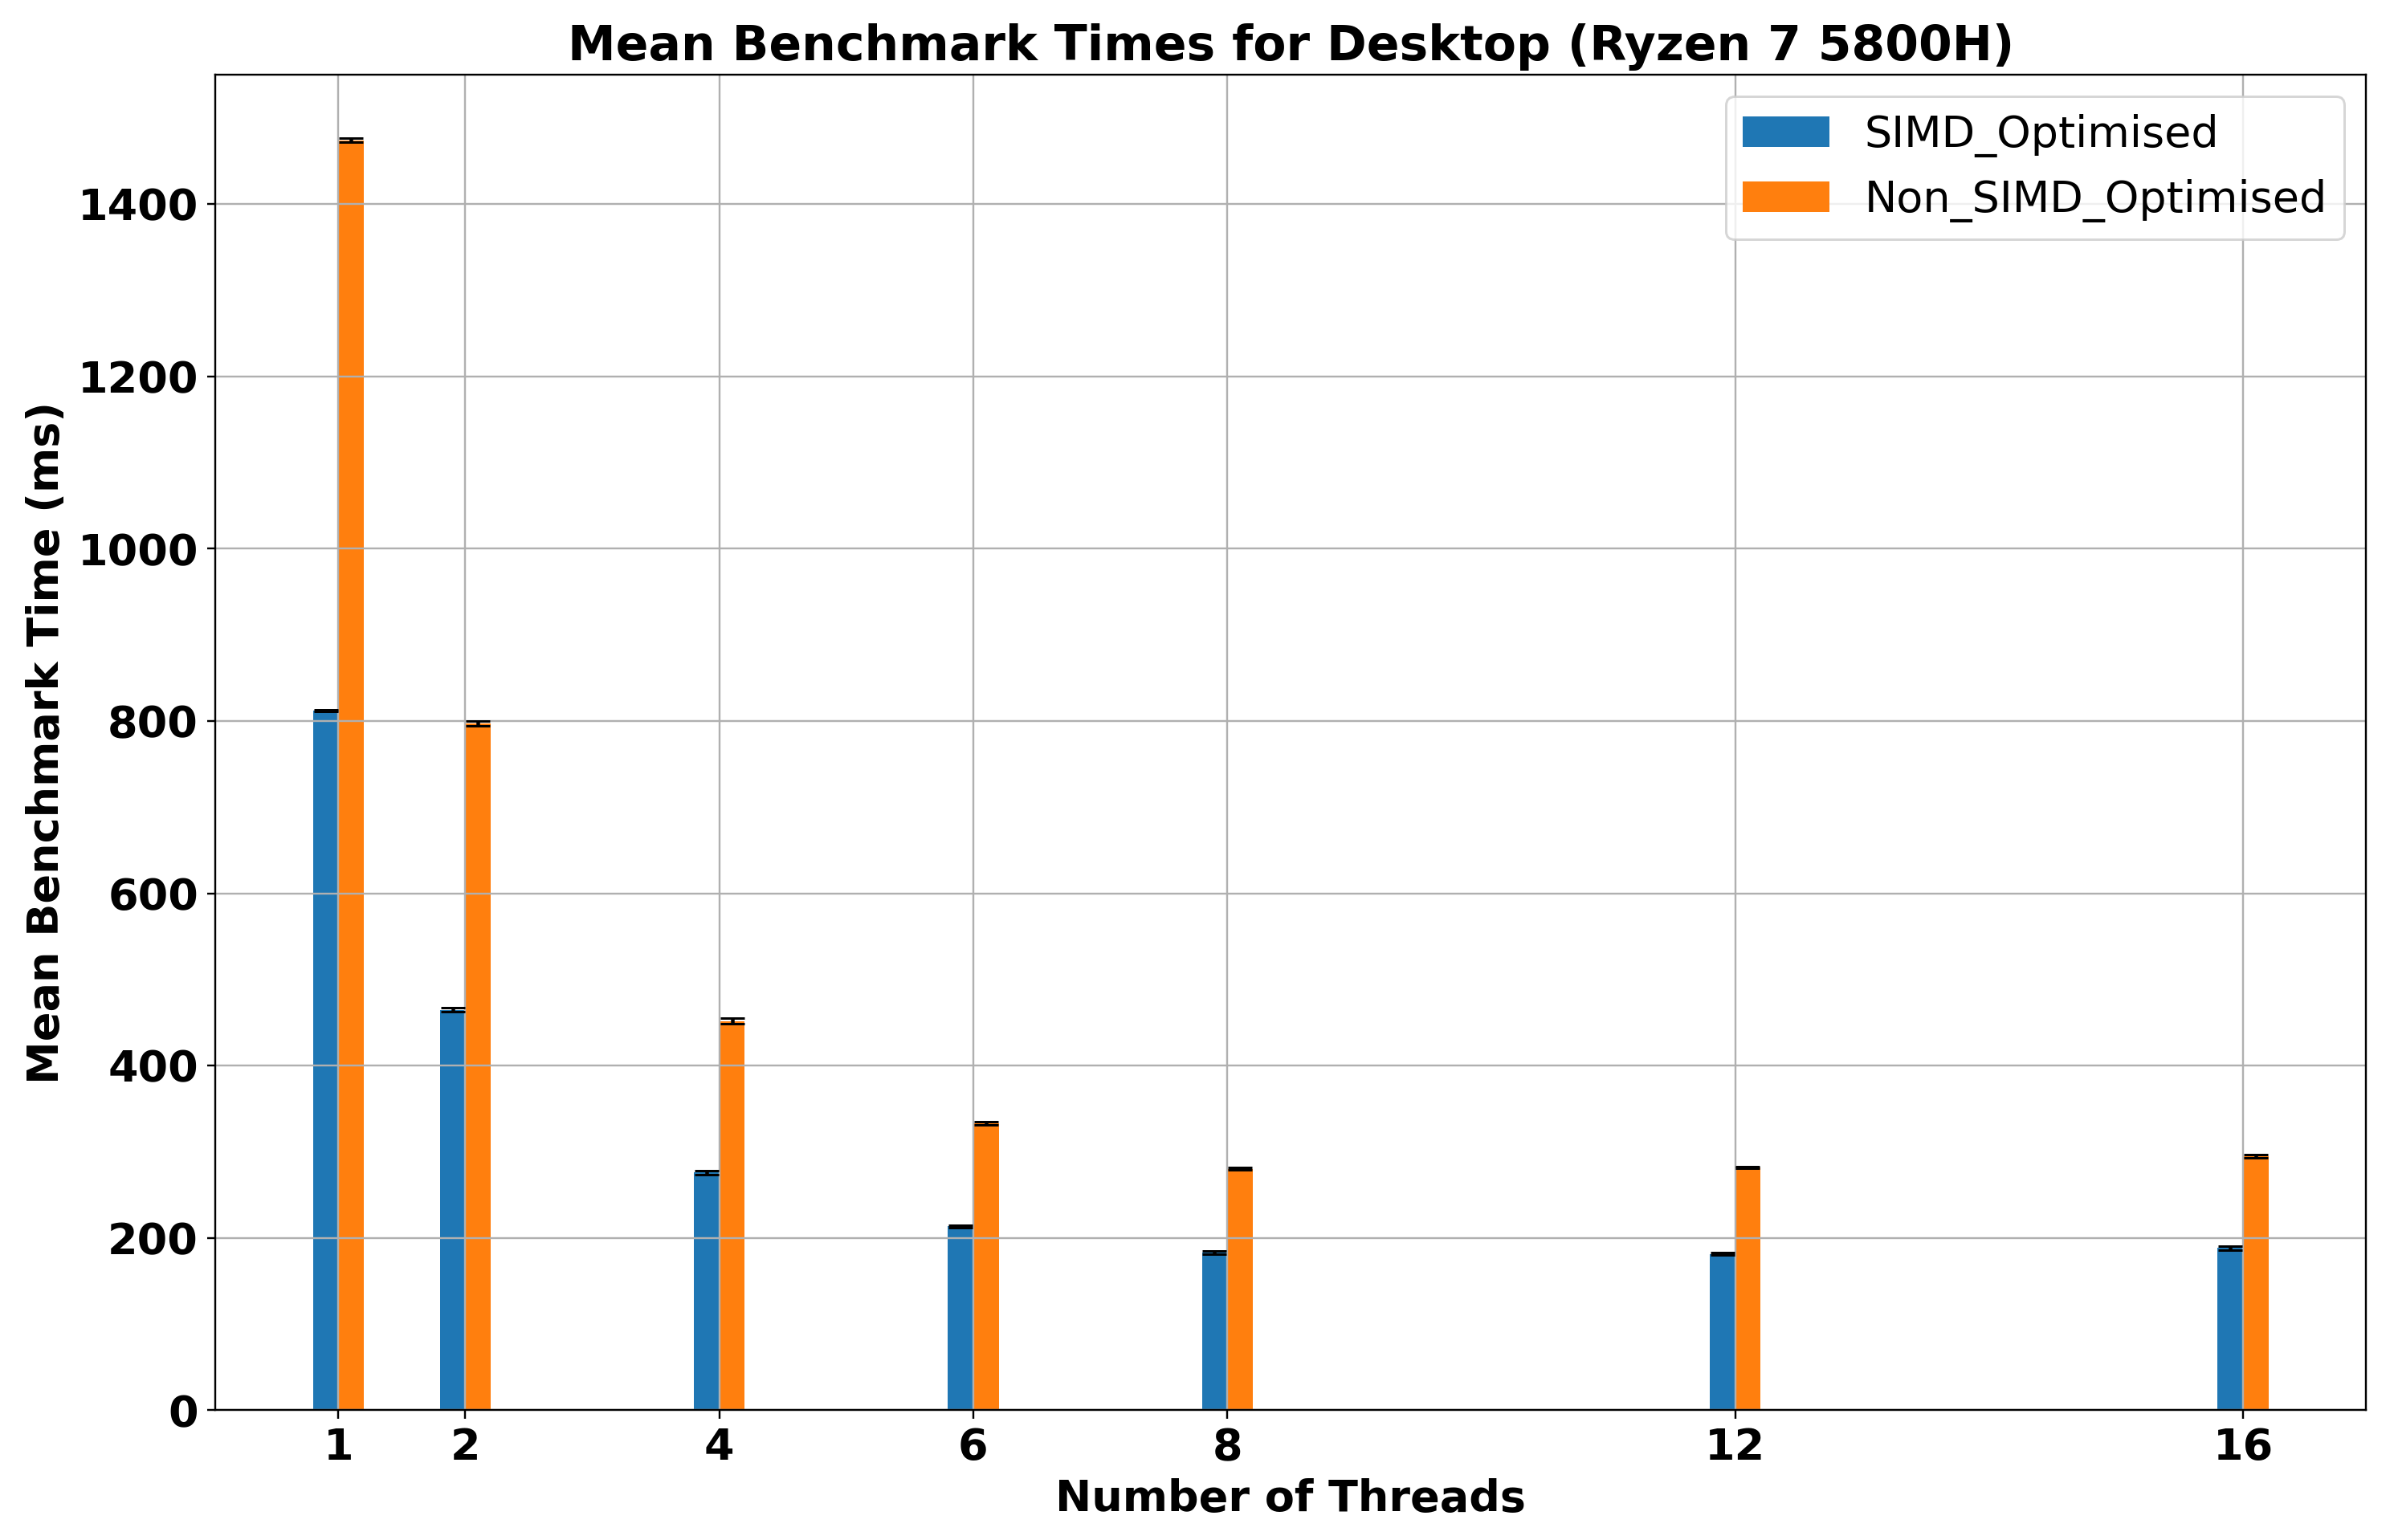
\includegraphics[width=1\textwidth, height=20cm]{~/Documents/Part_D_Modules/Individual_Project/Individual_report/figures/mobilenet_desktop.png} % Adjust the path and width as needed
	\caption{Mean benchmark plot of results collected from \texttt{x86} processor(in milliseconds). (Lower is better).}
	\label{fig:mobilenet_desktop_plot} % Use this label to reference the figure
\end{figure}

\begin{figure}[htbp] % Positioning preference: here, top, bottom, page
	\centering
	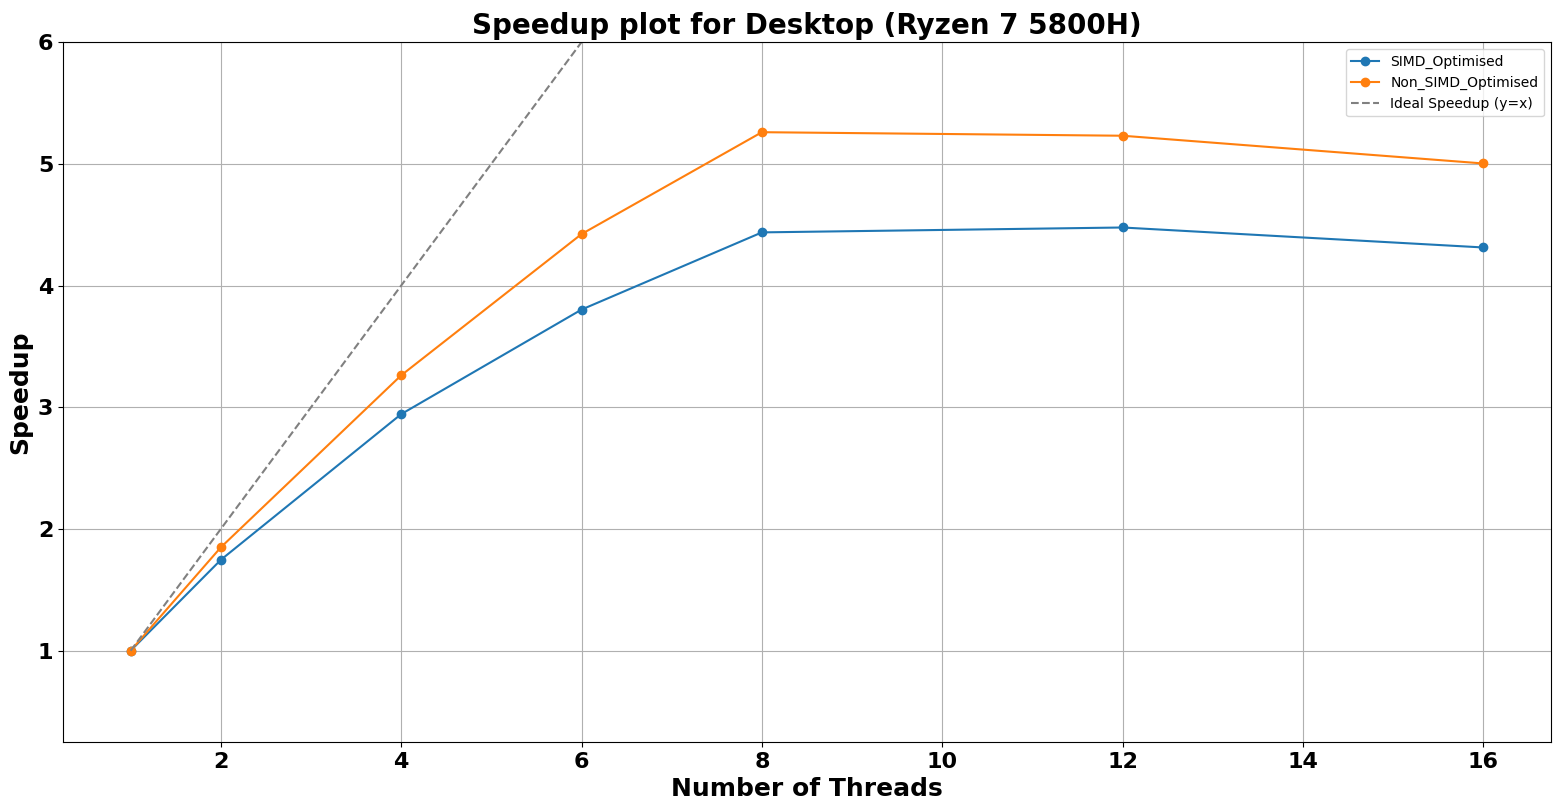
\includegraphics[width=1\textwidth, height=20cm]{~/Documents/Part_D_Modules/Individual_Project/Individual_report/figures/mobilenet_desktop_speedup.png} % Adjust the path and width as needed
	\caption{Speedup plot comparing the two solutions with results collected from \texttt{x86} processor. (Higher is better).}
	\label{fig:mobilenet_desktop_speedup} % Use this label to reference the figure
\end{figure}

The mean benchmark time of the original \texttt{MobileNet} application\cite{mobilenet_repo} was 1474.2 ms(using the \texttt{-O3} optimisation flag). The benchmark time using the maximum threads(16) with SIMD was 188.24ms and without SIMD it was 294.68ms. The SIMD optimisations are turned on and off as shown in listing  ~\ref{lst:mobilenet_parallel}. This presents a drastic reduction in run time of 87.2\% and 80.0\% for the SIMD and non-SIMD solutions respectively. Using multi-threading on the desktop processor yielded exceptional results and a dramatic improvement of the application. The results also indicate a performance degradation when using threads greater than 8 which is the maximum physical cores on the system. Both of the solutions produced a slight degradation of performance when going from 8 to 16 threads, suggesting once again the virtual cores from SMT did not yield in performance gains. 

The performance on the Raspberry Pi devices was a little more nuanced. The results of having different parallel regions and SIMD optimisations turned on or off were compared. The plots have the following legends:

\begin{enumerate}
	\item \texttt{3\_Parallel\_Regions\_SIMD}: all three functions \texttt{ConvLayer::forward}, \texttt{BatchNormalLayer::forward} and \texttt{ConvLayer::Addpad} have been parallelised with SIMD optimisations.
	\item \texttt{3\_Parallel\_Regions}: all three functions \texttt{ConvLayer::forward}, \texttt{BatchNormalLayer::forward} and \texttt{ConvLayer::Addpad} have been parallelised without SIMD optimisations.
	\item \texttt{2\_Parallel\_Regions\_SIMD}: only two functions \texttt{ConvLayer::forward} and \texttt{BatchNormalLayer::forward} have been parallelised with SIMD optimisations.
	\item \texttt{2\_Parallel\_Regions}: only two functions \texttt{ConvLayer::forward} and \texttt{BatchNormalLayer::forward} have been parallelised without SIMD optimisations.
\end{enumerate}

The results for Raspberry Pi 5 are shown in figures ~\ref{fig:mobilenet_rpi5_plot} and ~\ref{fig:mobilenet_rpi5_speedup}. The results for Raspberry Pi 4 are shown in figures ~\ref{fig:mobilenet_rpi4_plot} and ~\ref{fig:mobilenet_rpi4_speedup}. 

\begin{figure}[htbp] % Positioning preference: here, top, bottom, page
	\centering
	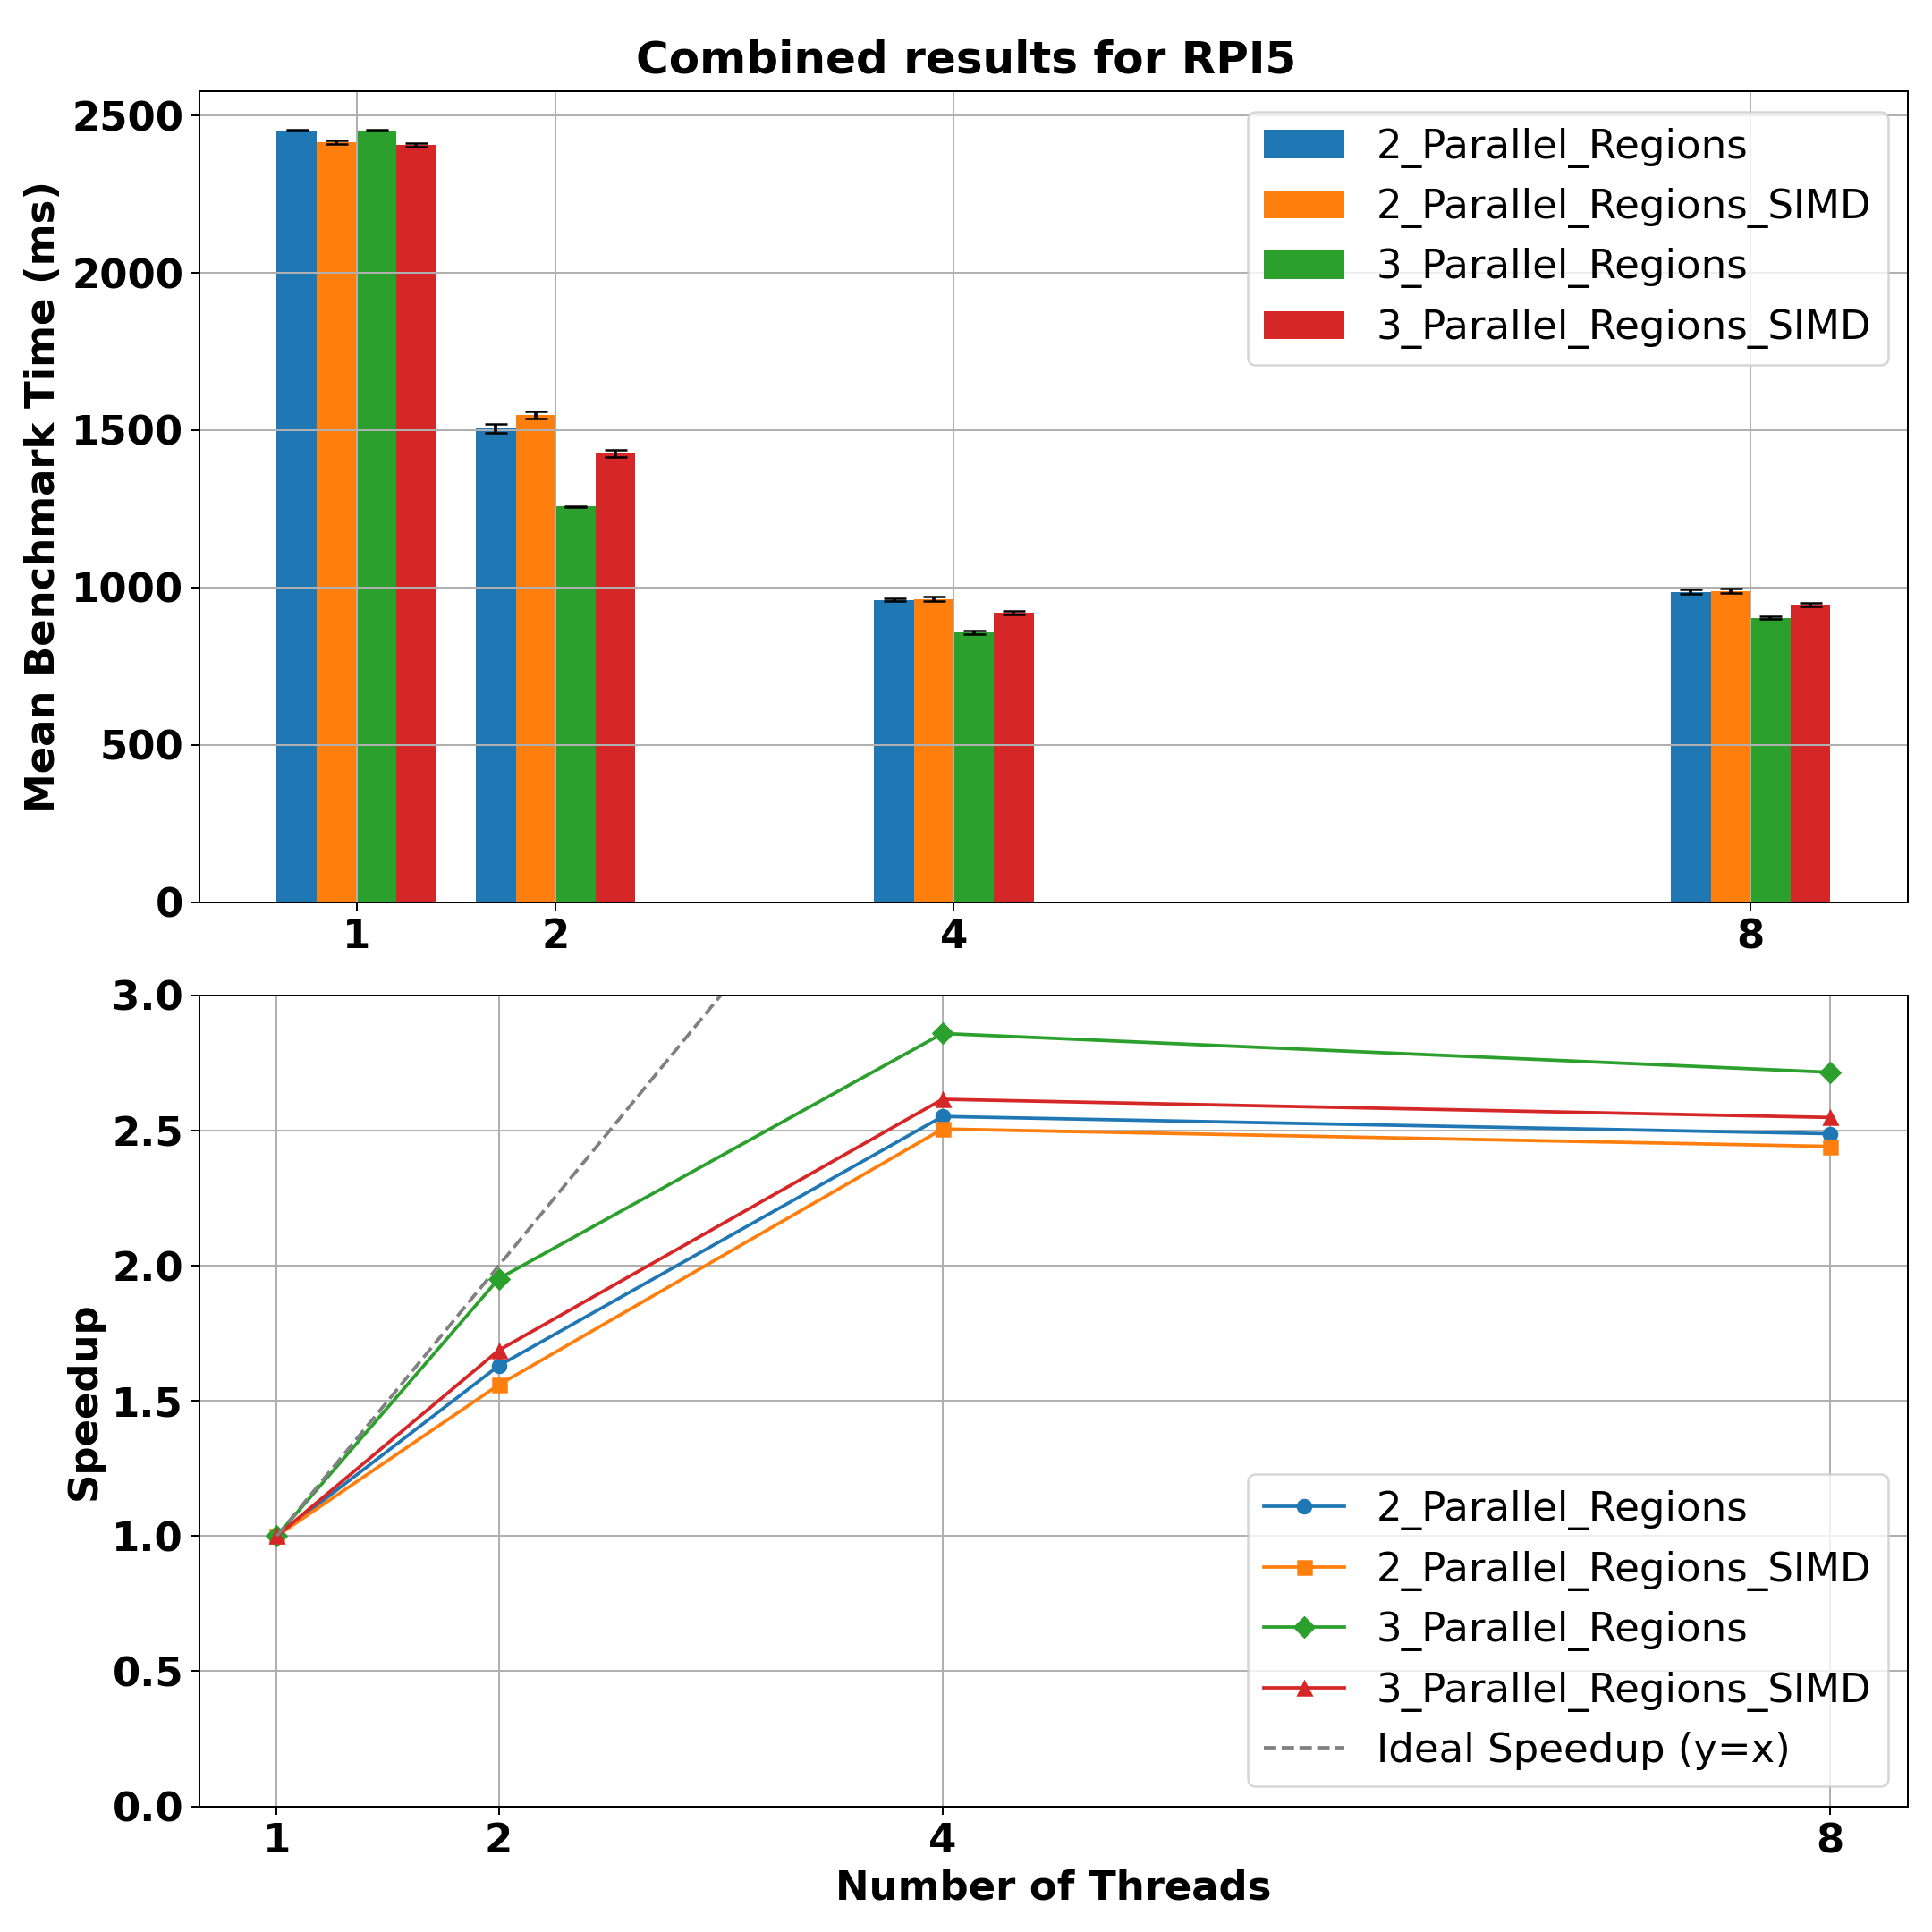
\includegraphics[width=1\textwidth, height=20cm]{~/Documents/Part_D_Modules/Individual_Project/Individual_report/figures/mobilenet_rpi5.png} % Adjust the path and width as needed
	\caption{Mean benchmark plot of results collected from \texttt{Cortex A-76} processor(in milliseconds). (Lower is better).}
	\label{fig:mobilenet_rpi5_plot} % Use this label to reference the figure
\end{figure}

\begin{figure}[htbp] % Positioning preference: here, top, bottom, page
	\centering
	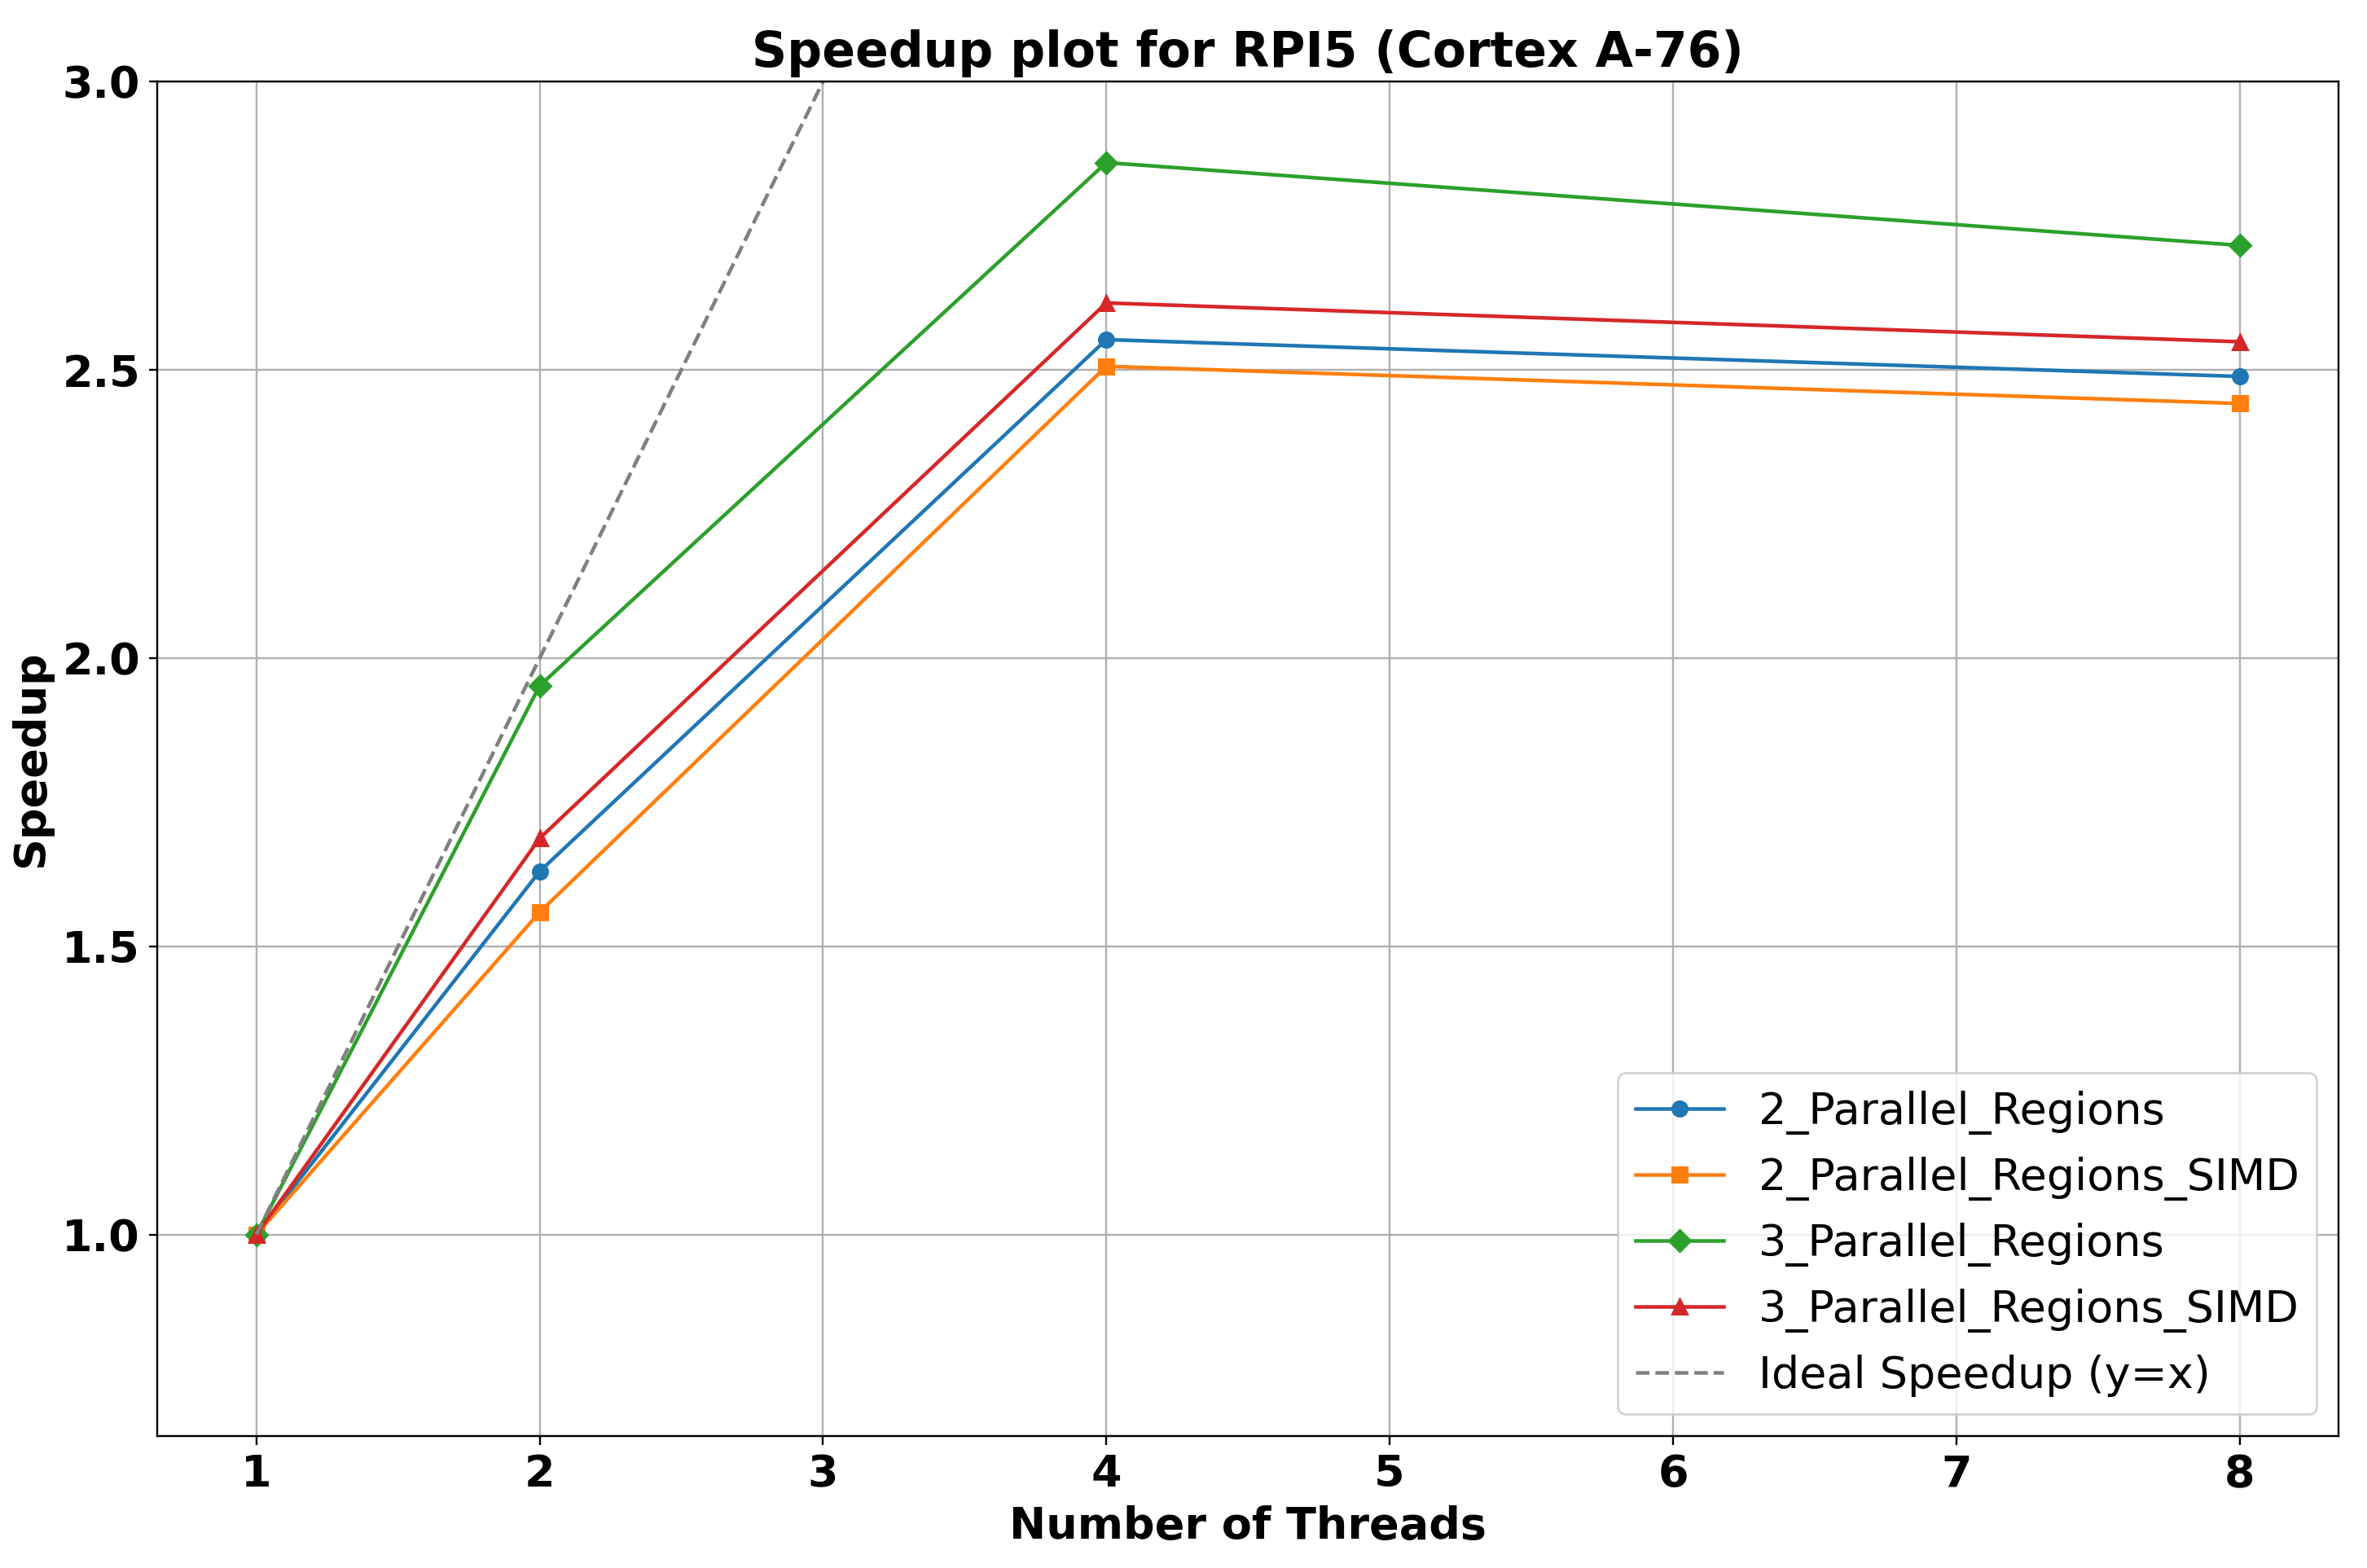
\includegraphics[width=1\textwidth, height=20cm]{~/Documents/Part_D_Modules/Individual_Project/Individual_report/figures/mobilenet_rpi5_speedup.png} % Adjust the path and width as needed
	\caption{Speedup plot comparing different solutions with results collected from \texttt{Cortex A-76} processor. (Higher is better).}
	\label{fig:mobilenet_rpi5_speedup} % Use this label to reference the figure
\end{figure}

\begin{figure}[htbp] % Positioning preference: here, top, bottom, page
	\centering
	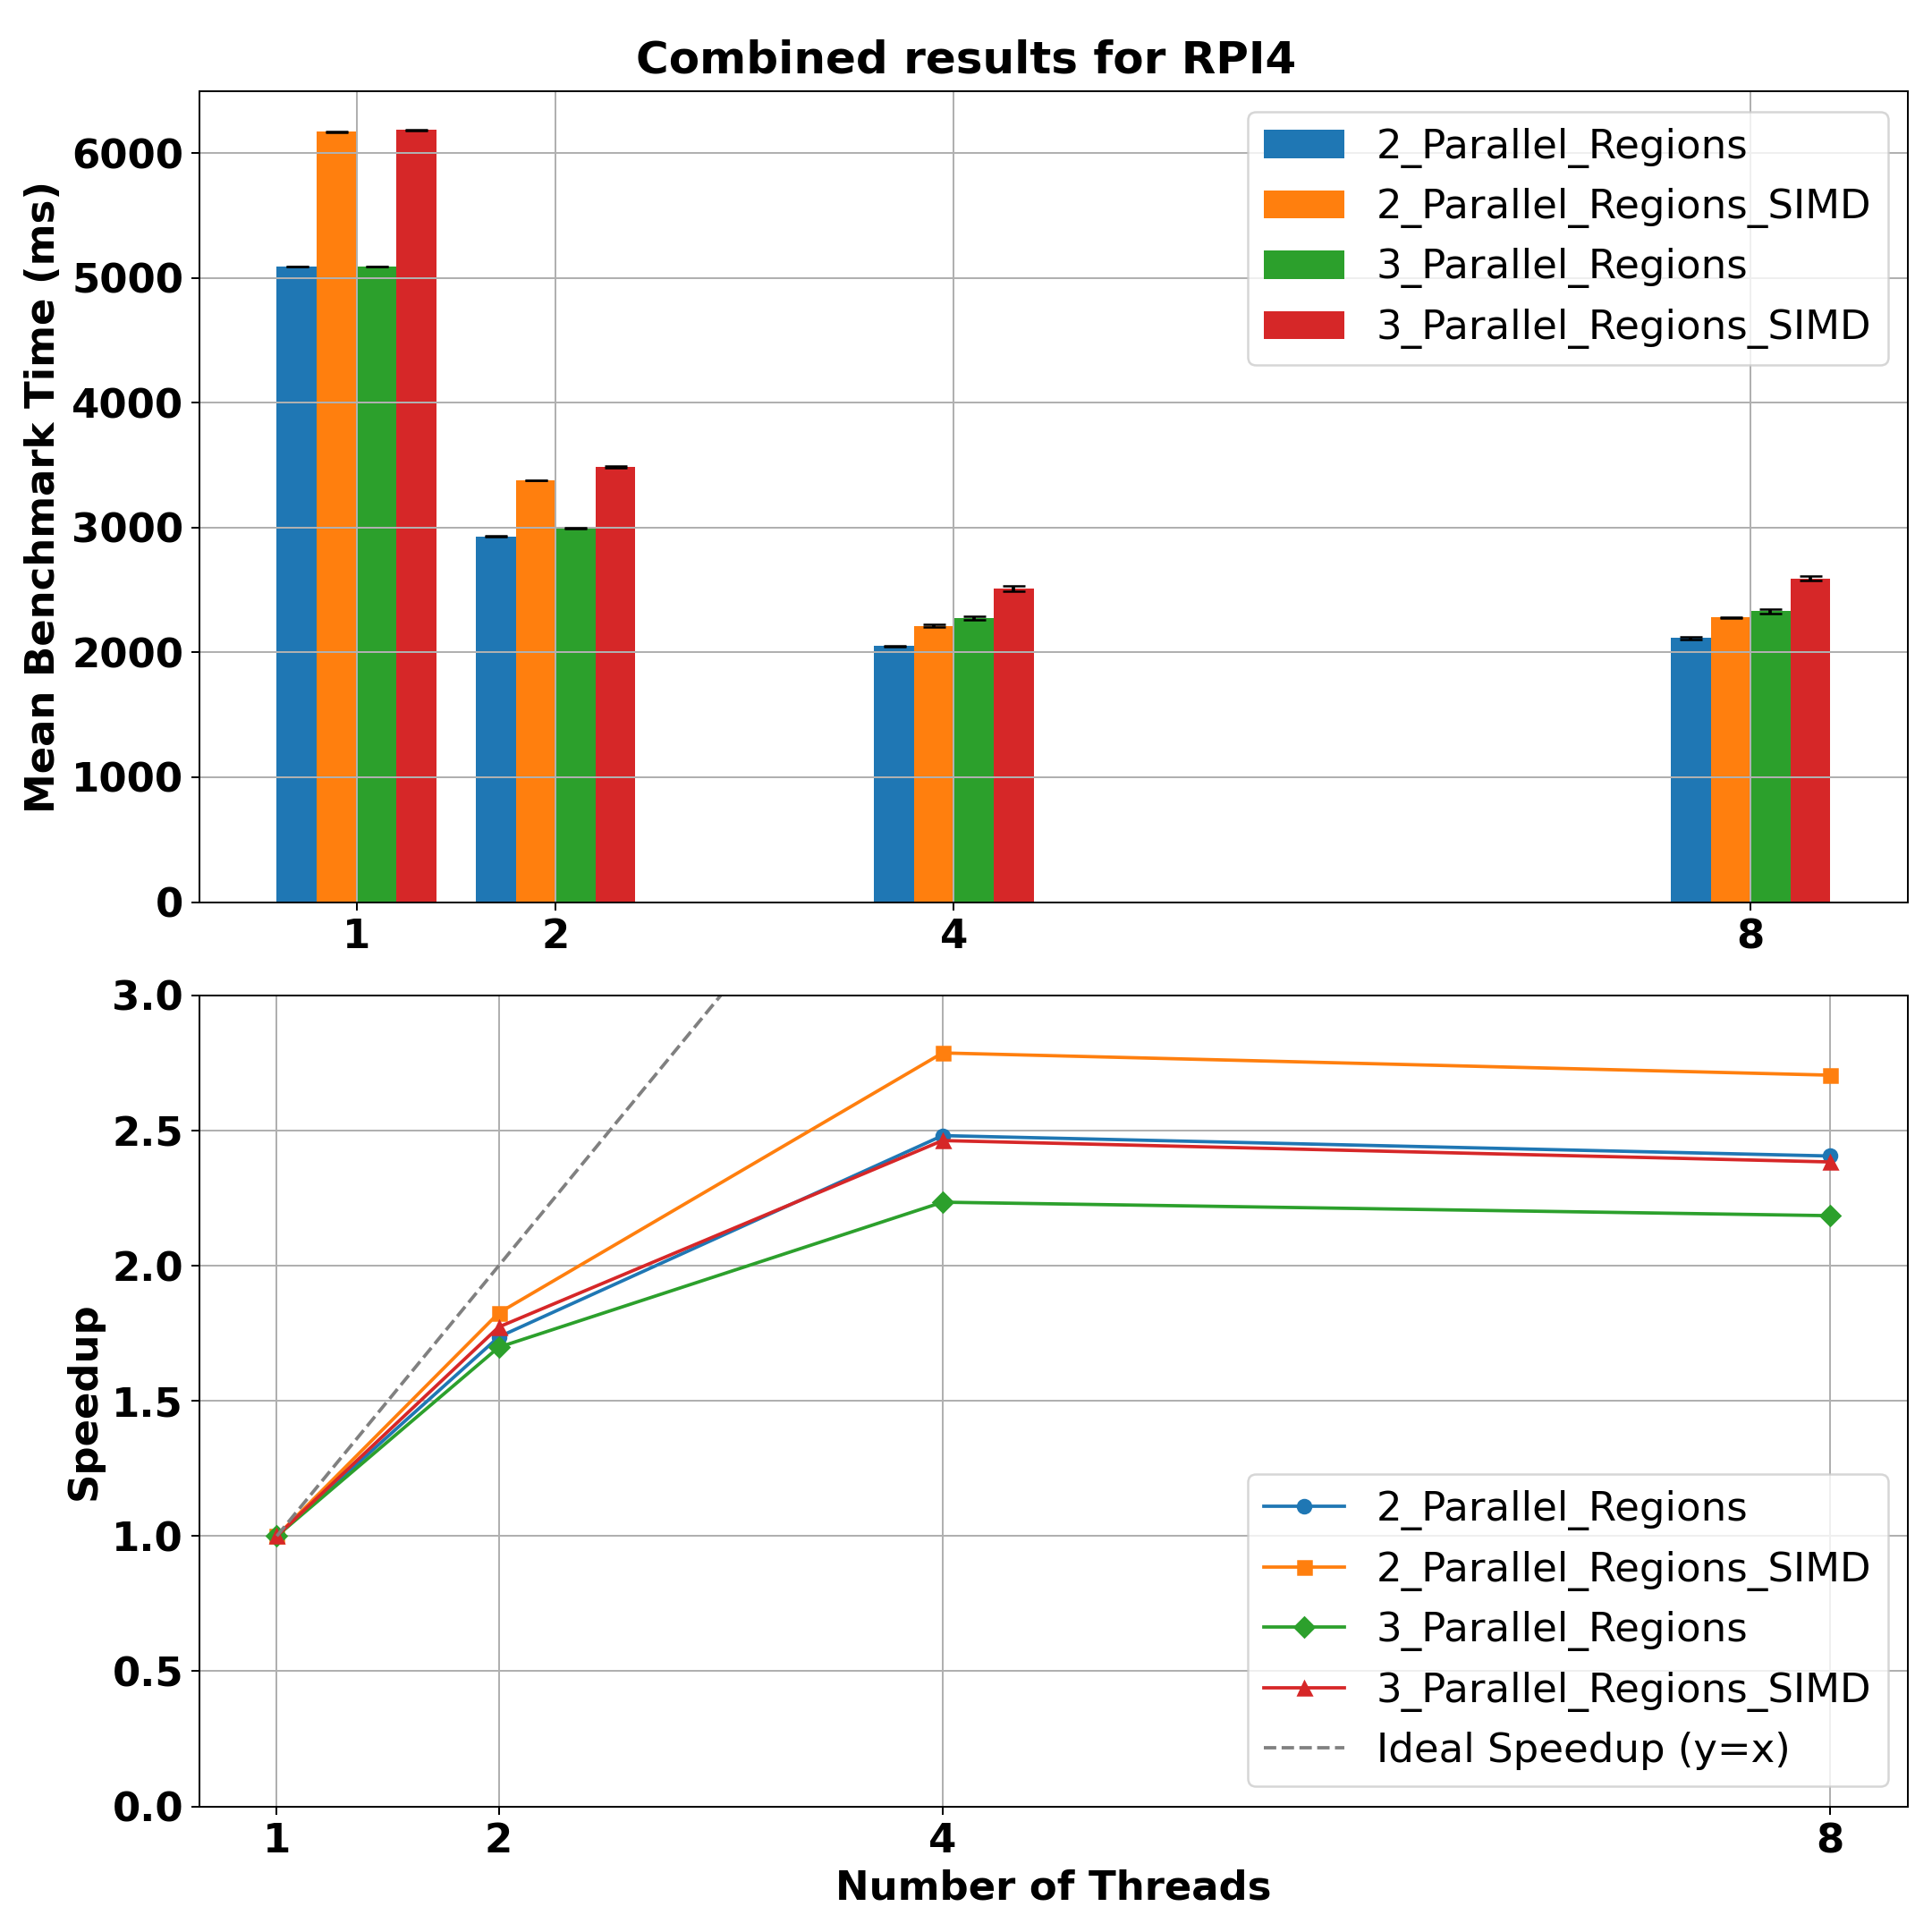
\includegraphics[width=1\textwidth, height=20cm]{~/Documents/Part_D_Modules/Individual_Project/Individual_report/figures/mobilenet_rpi4.png} % Adjust the path and width as needed
	\caption{Mean benchmark plot of results collected from \texttt{Cortex A-72} processor(in milliseconds). (Lower is better).}
	\label{fig:mobilenet_rpi4_plot} % Use this label to reference the figure
\end{figure}

\begin{figure}[htbp] % Positioning preference: here, top, bottom, page
	\centering
	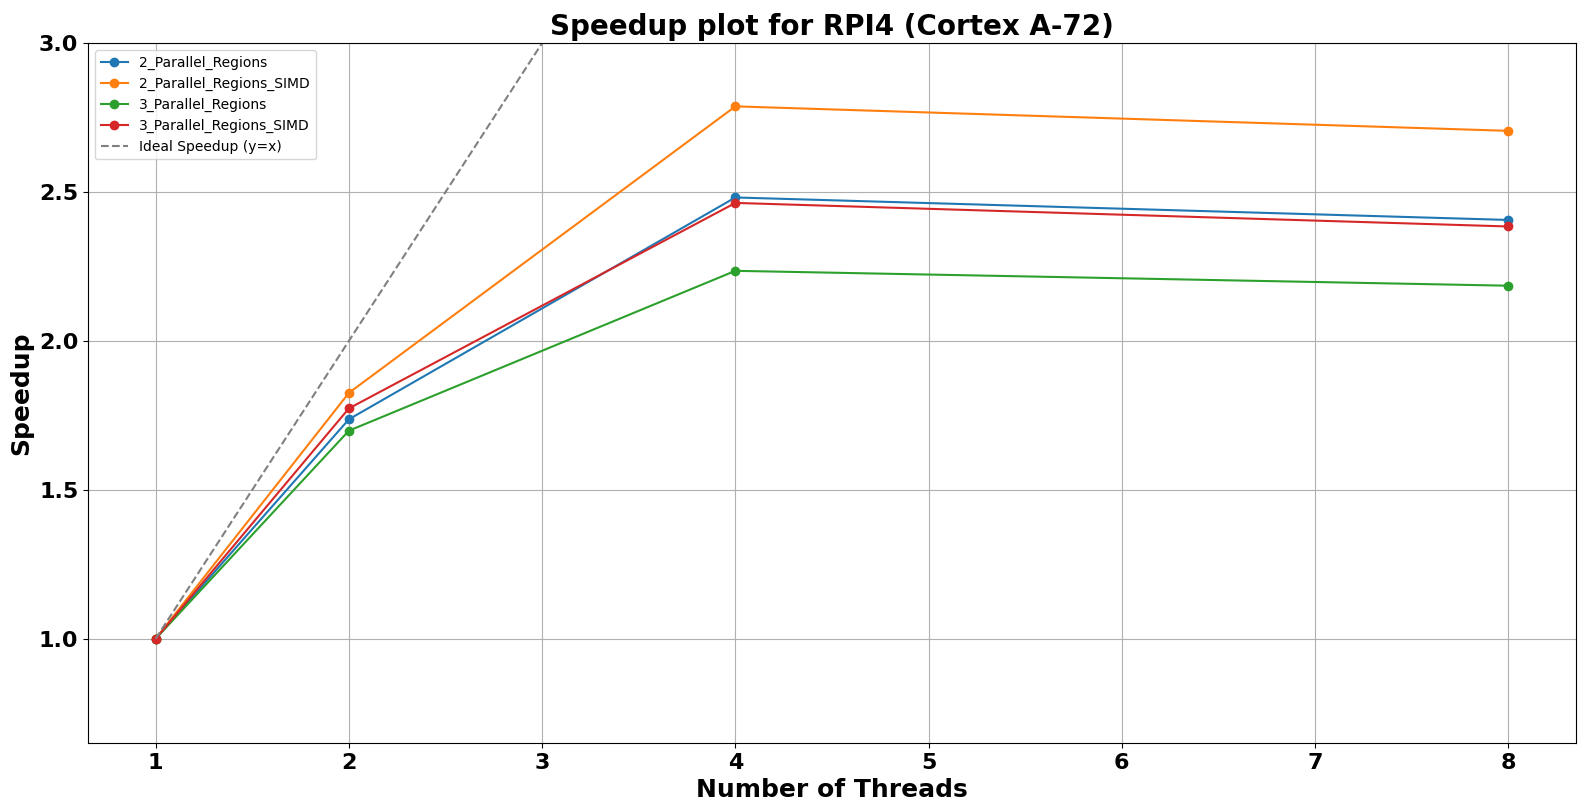
\includegraphics[width=1\textwidth, height=20cm]{~/Documents/Part_D_Modules/Individual_Project/Individual_report/figures/mobilenet_rpi4_speedup.png} % Adjust the path and width as needed
	\caption{Speedup plot comparing different solutions with results collected from \texttt{Cortex A-72} processor. (Higher is better).}
	\label{fig:mobilenet_rpi4_speedup} % Use this label to reference the figure
\end{figure}